\documentclass[parskip=full,11pt,twoside]{scrartcl}
\usepackage[utf8]{inputenc}

\title{Blockchain-basiertes E-Voting}
\author{Artem Vasilev, Achim Kriso, Philipp Schaback, Tim Fröhlich, David Schuldes}

% section numbers in margins:
\renewcommand\sectionlinesformat[4]{\makebox[0pt][r]{#3}#4}

% header & footer
\usepackage{scrlayer-scrpage}
\lofoot{\today}
\refoot{\today}
\pagestyle{scrheadings}

\usepackage[sfdefault,light]{roboto}
\usepackage[T1]{fontenc}
\usepackage[german]{babel}
\usepackage[yyyymmdd]{datetime} % must be after babel
\renewcommand{\dateseparator}{-} % ISO8601 date format
\usepackage{hyperref}
\usepackage{amsmath} % for $\text{}$
\usepackage[nameinlink]{cleveref}
\crefname{figure}{Abb}{Abb}
\usepackage[section]{placeins}
\usepackage{xcolor}
\usepackage{graphicx}
\hypersetup{
	pdftitle={Pflichtenheft},
	bookmarks=true,
}
\usepackage{csquotes}
\usepackage{float}

\usepackage{pflichtenheft}
\usepackage[nopostdot]{glossaries}
\makeglossaries
\newglossaryentry{Benutzer}{name={Benutzer},description={
Eine Person die mit der Software interagiert.
}}
	
\newglossaryentry{Wahl}{name={Wahl},description={
Eine Sammlung von Stimmen für die Bestimmung eines Kandidaten.
}}
		
\newglossaryentry{Waehler}{name={Wähler},description={
Person die bei einer Wahl einen bestimmten Kandidaten wählt und die hierfür nötigen Berechtigungen hat.
}}
			
\newglossaryentry{Kandidat}{name={Kandidat}, plural=Kandidaten, description={
Eine Entität, für die ein Wähler bei einer Wahl \glslink{Stimme}{stimmen} kann.
}}
				
\newglossaryentry{Stimme}{name={Stimme}, plural=Stimmen,description={
Eine Zähleinheit, die im \gls{Auszaehlungsverfahren} zur Ermittlung des Wahlergebnisses benutzt wird.
}}

\newglossaryentry{Datenbank}{name={Datenbank}, plural=Datenbanken, description={
Ein Elektronisches System zur Datenverwaltung.
}}

\newglossaryentry{Auszaehlungsverfahren}{name={Auszählungsverfahren},description={
Eine Methode um zu bestimmen, welcher Kandidat bei einer Wahl gewonnen hat.
}}

\newglossaryentry{Absolute-Mehrheitswahl}{name={Absolute Mehrheitswahl},description={
Auszählungsverfahren, bei dem der Kandidat gewinnt, der über 50\% der Stimmen hat. Ansonsten hat niemand gewonnen.
Ein Wähler kann seine Stimme genau einmal abgeben und für genau einen Kandidaten Stimmen.
}}

\newglossaryentry{Relative-Mehrheitswahl}{name={Relative Mehrheitswahl},description={
Auszählungsverfahren, bei dem der Kandidat mit den meisten Stimmen gewinnt.
Ein Wähler kann seine Stimme genau einmal abgeben und für genau einen Kandidaten Stimmen.
}}

\newglossaryentry{Instant-Runoff-Voting}{name={Instant-Runoff-Voting},description={
Auszählungsverfahren, bei dem der Wähler die Kandidaten nach Präferenz ordnet. Sei n die Anzahl der zur Auswahl stehenden Kandidaten, das Verfahren ist für Wahlen mit 3 oder mehr Kandidaten geeignet:
\begin{enumerate}
	\item Jeder Wähler kann jedem Kandidaten einen Wert von 1 bis n zuweisen. Werte düfen nicht mehrfach vergeben werden. Kandidaten müssen nicht bewertet werden.
	\item Bei der Auszählung wird bestimmt welcher Kandidat die wenigsten Stimmen mit Wert 1 bekommen hat. Dieser Kandidat wird dann aus allen Listen entfernt. Die Werte der Kandidaten auf den nachfolgenden Plätzen werden jeweils um 1 abgezogen.
	\item Schritt 2 wird so lange wiederholt bis nur noch 2 Kandidaten übrig sind. Der Kandidat mit den meisten ersten Stimmen hat gewonnen.
\end{enumerate}
}}

\newglossaryentry{Benutzeroberflaeche}{name={Benutzeroberfläche},description={
Grafische Benutzerschnittstelle zu einem Computer, welche eine leichte und intuitiver Benutzung der Software ermöglicht.
}}

\newglossaryentry{Konfigurationsmenu}{name={Konfigurationsmenü},description={
Die \gls{Benutzeroberflaeche} des \glslink{Wahlleiter}{Wahlleiters} in der er eine \gls{Wahl} \glslink{Konfiguration}{konfigurieren} kann.
}}

\newglossaryentry{Zertifikat}{name={Zertifikat}, plural=Zertifikate,description={
Digitaler Datensatz, der die Authentizität und Integrität von Personen oder Objekten durch kryptografische Verfahren nachweist.
}}

\newglossaryentry{Blockchain}{name={Blockchain},description={
Datenbanktechnologie bei der die einzelnen Datensegmente verknüpft werden um so Eigenschaften wie Unveränderbarkeit und Dezentralisierung zu erreichen.
}}

\newglossaryentry{Ledger}{name={Blockchain-Ledger},description={
Datenbank in einer Blockchain, welche alle Transaktionen, die auf der Blockchain ausgeführt wurden, enthält. In dem Kontext unserer Wahl sind die Transaktionen einzelne Stimmen. Jeder Peer in dem Netzwerk besitzt einen Ledger.
}}

\newglossaryentry{Netzwerk}{name={Blockchain-Netzwerk},description={
Menge an verknüpften \glslink{Peer}{Peers}, die zusammen einen synchronierten \gls{Ledger} verwalten.
}}

\newglossaryentry{Peer}{name={Peer},description={
Computer der eine Kopie des Ledgers enthält, diese mit anderen Peers synchronisiert und eine Schnittstelle zwischen Chaincode und Software bereitstellt.
}}

\newglossaryentry{Chaincode}{name={Chaincode},description={
Programme die auf der Blockchain laufen und als Schnittstelle eines Peers zur Blockchain dienen.
}}

\newglossaryentry{Logdatei}{name={Logdatei},description={
Datei welche alle Ereignisse (Informationen, Warnungen und Fehler) in einem System protokolliert.
}}

\newglossaryentry{Linux}{name={Linux},description={
Beliebtes Unix-like Betriebssystem.
}}

\newglossaryentry{Double-Spending-Problem}{name={Double-Spending-Problem},description={
Die mehrfache, erfolgreiche Abgabe einer Stimme in einem Wahlsystem. Die erfolgreiche \gls{Stimmabgabe} darf pro \gls{Waehler} maximal einmal erfolgen.
}}

\newglossaryentry{Wahlleiter}{name={Wahlleiter},description={
Administrator der Wahl, legt die Einstellungen, Wähler und Kandidaten der Wahl fest.
}}

\newglossaryentry{Dateibrowser}{name={Dateibrowser},description={
Programm, welches dem User eine Benutzeroberfläche zum verwalten von Dateien bietet.
}}

\newglossaryentry{Konfiguration}{name={Konfiguration},description={
Feste Belegung der einstellbaren Eigenschaften eines Systems (hier i.d.R die Wahl).
}}

\newglossaryentry{Benutzerdaten}{name={Benutzerdaten},description={
Daten, die für einen Benutzer spezifisch sind. Beispielsweise Name, Geburtsdatum, Herkunftsland und Geschlecht.
}}

\newglossaryentry{Wahlberechtigung}{name={Wahlberechtigt},description={
Vom Wahlleiter als Wähler zugelassen und somit im Besitz eines gültigen Zertifikats zur Authentifizierung.
}}

\newglossaryentry{Stimmabgabe}{name={Stimmabgabe},description={
Hat ein Wähler über die Benutzeroberfläche einen Kandidaten gewählt bestätigt er seine Auswahl. Seine Stimme wird dann vom Klienten an das Blockchain-Netzwerk gesendet. Sofern die Stimme gültig ist wird sie in den Ledger eingetragen. Ansonsten wird die Stimme verworfen. Eine Stimme ist genau dann gültig wenn der Wähler sich als Wahlberechtigt authentifizieren konnte und seine Stimme noch nicht abgegeben hat.
}}

\newglossaryentry{Stimmenauszaehlung}{name={Stimmenauszählung},description={
Das Auslesen der Stimmen aus der Blockchain um zu bestimmen wer die Wahl gewonnen hat. Dabei wird beachtet welches Wahlverfahren für die Wahl definiert wurde.
}}

\newglossaryentry{Wahl-Ende}{name={Wahl-Ende},description={
Sobald die in der Wahl Konfiguration eingestellte Endbedingung erfüllt ist, beendet sich die Wahl. Es ist nicht mehr möglich gültige Stimmen abzugeben. Die Ergebnisse der Wahl werden für jeden Wähler auf dessen Klienten ausgewertet und in der GUI angezeigt.
}}

\newglossaryentry{Klient}{name={Klient},description={
Das Programm das auf den Computern der Wählern und des Wahlleiter läuft. Es stellt die GUI bereit und verwaltet die Kommunikation mit dem \gls{Netzwerk}.
}}

\newglossaryentry{Wahlstand}{name={Wahlstand},description={
Das Auswertungsergebnis der Wahl, bei dem alle bisher erfolgreich abgegebenen Stimmen ausgezählt werden.
}}

\newglossaryentry{Latenz}{name={Latenz},description={
Die zeitliche Differenz vom Abschicken einer Anfrage zum Empfangen der Antwort.
}}

\newglossaryentry{Consensus-Verfahren}{name={Consensus-Verfahren},description={
Eine Methode um die valide Transaktionen in einer \gls{Blockchain} zu verifizieren. Beim Consensus-Verfahren entscheided jeder \gls{Peer} ob eine Transaktion gültig ist. Wenn genug \gls{Peers} eine Transaktion akzeptieren wird diese Transaktion in den \gls{Ledger} geschrieben.
}}




\begin{document}
\maketitle

\pagebreak

\tableofcontents
\pagebreak
%%%%%%%%%%%%%%
\section{Produktübersicht}

Bei herkömmlichen E-Voting Lösungen gestaltet es sich als problematisch, Manipulation von Wahlergebnissen zu verhindern und den Wählern zu gewährleisten, dass ihre Stimme unverändert in die Wahl eingegangen ist. \\
Die Blockchain E-Voting Software löst diese Probleme mithilfe der Blockchain-Technologie. \\
Sobald ein Wähler seine Stimme abgibt wird sie im \gls{Ledger} gespeichert und kann nicht mehr verändert werden. Über diesen Weg garantiert die Software, dass seine Stimme nicht verloren geht und unverändert gespeichert wurde.

\section{Zielbestimmung}

\subsection{Musskriterien}

\criterium{Unterstützte Wahlformen}{crt:vote-formats}
Die Software unterstützt das Mehrheitswahl-Prinzip. Es ist möglich eine Wahl aufzusetzen, bei der der Gewinner nach dem Prinzip der 
%\glslink{Absolute-Mehrheitswahl}{Absoluten Mehrheitswahl} oder
% Wenn dies in den Sollriterien erneut aufgefasst wird sollte es nicht in den Musskriterien stehen
\glslink{Relative-Mehrheitswahl}{Relativen Mehrheitswahl} ermittelt wird.

\criterium{Erstellung von Wahl}{crt:create}
Ein \gls{Wahlleiter} kann eine \gls{Wahl} über seine \gls{Benutzeroberflaeche} \glslink{Konfiguration}{konfigurieren}.
Wenn eine \gls{Wahl} gestartet ist können nur \gls{Waehler}, die als \glslink{Wahlberechtigung}{wahlberechtigt} authentifiziert sind, die \gls{Wahl} in ihrer \gls{Benutzeroberflaeche} sehen.

\criterium{Rückmeldung bei Stimmabgabe}{crt:vote-feedback}
Wenn ein \gls{Waehler} seine \gls{Stimme} abgegeben hat wird er über seine \gls{Benutzeroberflaeche} informiert, ob seine \gls{Stimmabgabe} erfolgreich war oder nicht. Eine \gls{Stimmabgabe} ist genau dann erfolgreich, wenn die \gls{Stimme} im \gls{Ledger} eingetragen wurde.

\criterium{Stimmenübermittlung}{crt:send}
Ist die \gls{Stimmabgabe} eines \glslink{Waehler}{Wählers} erfolgreich garantiert die Software, dass seine \gls{Stimme} unverändert zum \gls{Ledger} hinzugefügt wurde.

\criterium{Stimmenauszählung}{crt:count}
Sobald eine \gls{Wahl} \glslink{Wahl-Ende}{beendet} ist werden alle erfolgreich \glslink{Stimmabgabe}{abgegebenen} Stimmen mit einem \gls{Auszaehlungsverfahren} ausgezählt. Das \gls{Auszaehlungsverfahren} wird bei der \glslink{Konfiguration}{Wahlkonfiguration} festgelegt.

\criterium{Graphische Benutzeroberfläche für Wahlleiter}{crt:gui-es}
Der \gls{Wahlleiter} kann über seine \gls{Benutzeroberflaeche} eine Wahl \glslink{Konfiguration}{konfigurieren}. Ist eine \gls{Wahl} gestartet wird der aktuelle \gls{Wahlstand} auf seiner \gls{Benutzeroberflaeche} angezeigt. Ist die Wahl \glslink{Wahl-Ende}{beendet} wird das Ergebnis der \glslink{Stimmenauszaehlung}{Auszählung} auf der \gls{Benutzeroberflaeche} angezeigt.

\criterium{Graphische Benutzeroberfläche für Wähler}{crt:gui-voter}
Die \gls{Benutzeroberflaeche} des \glslink{Waehler}{Wählers} bietet Informationen über die \glslink{Kandidat}{Kandidaten}, erlaubt es für einen \glslink{Kandidat}{Kandidaten} zu stimmen und bietet Erklärungen zum Ablauf der Wahl.

\subsection{Sollkriterien}

\criteriumShould{Absolute Mehrheitswahl}{crt:absfptp}
Wahlen können mit dem \gls{Auszaehlungsverfahren} der \glslink{Absolute-Mehrheitswahl}{Absoluten Mehrheitswahl} ausgewertet werden. Die \gls{Absolute-Mehrheitswahl} ist dementsprechend eine Option die dem \gls{Wahlleiter} zur Verfügung gestellt wird.
Sollte zum Ende der Wahl keiner der Kandidaten 50\% erreicht haben gibt es keinen Gewinner.
In diesem Fall wird dem Wahlleiter die Möglichkeit geboten die Wahl erneut zu starten.

\criteriumShould{Speichern der Konfiguration}{crt:safeconf}
Der \gls{Wahlleiter} kann eine \gls{Konfiguration} in einer Datei abspeichern und wieder laden. Diese Funktionalität ist in dem \gls{Konfigurationsmenu} erreichbar. Das Laden einer solchen Datei überschreibt alle Informationen die schon in dem \gls{Konfigurationsmenu} eingegeben wurden.

\subsection{Kannkriterien}

\criteriumOptional{Instant-Runoff-Voting}{crt:irv}
Das \gls{Auszaehlungsverfahren} \gls{Instant-Runoff-Voting} kann benutzt werden um eine Wahl auszuwerten und wird dem \gls{Wahlleiter} zur Auswahl gestellt.

\criteriumOptional{Geheime Wahlen}{crt:secret}
Bereitstellung von Wahlen bei denen die Stimmen der Wähler für niemanden außer für den Wahlleiter einsehbar sind.
Das Wahlergebnis kann am Ende der Wahl vom Wahlleiter an die Wähler propagiert werden.

\criteriumOptional{Verteilung von Zugangsdaten}{crt:certdist}
Funktionalität die es dem \gls{Wahlleiter} erlaubt Zugangsdaten (Name und \gls{Zertifikat}) für die \gls{Wahl} per Email an die \gls{Waehler} zu verteilen

\criteriumOptional{Automatisches Wahlende}{crt:autoend}
Bestimmung einer weiteren Endbedingung bei der \glslink{Konfiguration}{Wahlkonfiguration} deren Erfüllung die \gls{Wahl} automatisch beendet.
Eine Wahl ist \glslink{Wahl-Ende}{beendet} wenn der bei der \glslink{Konfiguration}{Wahlkonfiguration} festgelegte Endzeitpunkt der Wahl erreicht ist, oder wenn die zusätzlich festgelegte Endbedingung erreicht ist.
Die zusätzlichen Endbedingungen sind:\\
Ein bei der \glslink{Konfiguration}{Wahlkonfiguration} festgelegter Prozentsatz an \glslink{Waehler}{Wählern} hat seine Stimme erfolgreich \gls{Stimmabgabe}{abgegeben}.\\
Ein \gls{Kandidat} hat einen bei der \glslink{Konfiguration}{Wahlkonfiguration} festgelegten Prozentsatz an insgesamt zugelassenen \glslink{Waehler}{Wählern} erreicht.

\subsection{Abgrenzungskriterien}
\criteriumNot{Unveränderbarkeit einer Stimme}{cst:nochange}
Sobald der \gls{Waehler} eine Stimme \glslink{Stimmabgabe}{abgegeben} hat, kann er diese nicht mehr ändern. Das gilt insbesondere auch wenn die \gls{Wahl} noch läuft.
\criteriumNot{Kein Speichern von Wahlverhalten}{cst:nomem}
Das Wahlverhalten (Die \glslink{Stimme}{Stimmen} eines \glslink{Waehler}{Wählers} in früheren \glslink{Wahl}{Wahlen}) eines \glslink{Waehler}{Wählers} ist nicht mehr nachvollziehbar, nachdem die \gls{Wahl} abgeschlossen ist.
\criteriumNot{Vertrauen in den Wahlleiter}{cst:trustes}
Die Legitimität der \gls{Wahl} basiert auf der Vertrauenswürdigkeit des \glslink{Wahlleiter}{Wahlleiters}. Da der \gls{Wahlleiter} alle \glslink{Zertifikat}{Zertifikate} besitzt, kann er sich für jeden \gls{Waehler} ausgeben und in dessen Namen wählen.
%%%%%%%%%%%
\section{Produkteinsatz}

\subsection{Anwendungsbereiche}
Durchführung von kleinen Wahlen oder Abstimmungen im Rahmen von Vereinen, Firmen oder Parlamenten.

\subsection{Zielgruppen}
\begin{enumerate}
  \item \gls{Waehler}
  \item \gls{Wahlleiter}
\end{enumerate}

\section{Produktumgebung}

\subsection{Software}
Das Programm soll für das Erstellen und Verwalten der \gls{Blockchain} das Hyperledger Fabric Framework verwenden, welches eine auf dem Consensus-Verfahren basierende Blockchain-Implementierung bietet.
Hierfür wird die Hauptanwendung in Java 7 geschrieben und das Hyperledger Fabric Java SDK verwendet. Für das erstellen von \glslink{Chaincode}{Chaincodes} soll Go verwendet werden.
Um die Funktionalität von Hyperledger Fabric zu gewährleisten wird ebenso eine Installation von GoLang benötigt.

\subsection{Hardware}
Es werden Computer für die \gls{Waehler} und den \gls{Wahlleiter} benötigt. Diese Computer müssen mit einer Internetverbindung ausgestattet sein und mindestens Java 7 installiert haben.

\subsection{Orgware}
\begin{enumerate}
\item Installation der Software, die für das Funktionieren von Hyperledger erforderlich ist. (siehe http://hyperledger-fabric.readthedocs.io/en/release-1.1/prereqs.html)
\item Anlegen des Netzwerks, wenn es keines gibt.
\end{enumerate}

\subsection{Schnittstellen}
Die \gls{Wahl} eines \glslink{Waehler}{Wählers} wird im \gls{Ledger} gespeichert und über das Netzwerk verteilt.

\section{Funktionale Anforderungen}

\functionality{Erstellung einer Wahl}{fnc:create}
\fulfills{crt:create}
\fulfills{crt:gui-es}
\fulfills{crt:safeconf}
Der \gls{Wahlleiter} kann eine neue \gls{Wahl} erstellen. Es existiert immer nur eine \gls{Wahl} zu einem Zeitpunkt.
Zudem kann eine Vorher abgespeicherte Wahlkonfiguration geladen werden. Hierbei öffnet sich das Konfigurationsmenü mit den geladenen Einstellungen in der \hyperref[fig:wlltr-done]{Überssichtsseite}.
Der \gls{Wahlleiter} wird durch die Erstellung geführt. Es sind folgende Schritte notwendig:

\functionality{Allgemeine Konfiguration der Wahl}{fnc:params}
\fulfills{crt:create}
\fulfills{crt:gui-es}
\fulfills{crt:secret}
Der \gls{Wahlleiter} legt den Namen und einen Beschreibungstext der \gls{Wahl} fest.
Er setzt den Start- und Endzeitpunkt der Wahl.

\functionality{Auswahl des Auszählungsverfahrens}{fnc:votesys}
\fulfills{crt:vote-formats}
\fulfills{crt:gui-es}
\fulfills{crt:absfptp}
\fulfills{crt:irv}
Die Festlegung eines \glslink{Auszaehlungsverfahren}{Auszählungsverfahrens} ist möglich. Es stehen die folgenden zur Verfügung:
\begin{itemize}
	\item \gls{Relative-Mehrheitswahl}
	\item \gls{Absolute-Mehrheitswahl}
	\item \gls{Instant-Runoff-Voting}
\end{itemize}

\functionality{Hinzufügen von Wählern}{fnc:voter-add}
\fulfills{crt:create}
\fulfills{crt:gui-es}
\fulfills{crt:certdist}
Der \gls{Wahlleiter} fügt die \gls{Waehler} mit ihrem Namen hinzu. Das System generiert automatisch die erforderlichen \glspl{Zertifikat}. Die \glspl{Zertifikat} werden im Netzwerk verteilt. Nur die hinzugefügten \gls{Waehler} sind zur Teilname berechtigt. \\
Der \gls{Wahlleiter} kann außerdem die \glspl{Zertifikat} per Email an die \gls{Waehler} senden. % Wie vermerkt man hier das das Teil des Kannkriteriums ist?

\functionality{Hinzufügen von Kandidaten}{fnc:candidate-add}
\fulfills{crt:create}
\fulfills{crt:gui-es}
Der \gls{Wahlleiter} fügt die \glslink{Kandidat}{Kandidaten} mit ihrem Namen hinzu. Es ist außerdem möglich jedem \glslink{Kandidat}{Kandidaten} eine Beschreibung zu geben, die den \glslink{Waehler}{Wählern} in ihrer \glslink{Benutzeroberflaeche}{GUI} angezeigt wird. Das System propagiert die \glslink{Kandidat}{Kandidaten} automatisch an das Netzwerk

\functionality{Exportieren der Wahlkonfiguration}{fnc:export}
\fulfills{crt:create}
\fulfills{crt:gui-es}
\fulfills{crt:safeconf}
Der \gls{Wahlleiter} hat die Möglichkeit seine vorgenommenen Einstellungen in einer Datei zu exportieren.
Es wird ein Dateibrowser geöffnet in welchem der Speicherort für die Konfigurationsdatei festgelegt werden kann.
Die gespeicherte Konfigurationsdatei beinhaltet alle Einstellungen der Wahl.

\functionality{Aktivierung der Wahl}{fnc:activate}
\fulfills{crt:create}
\fulfills{crt:gui-es}
Der \gls{Wahlleiter} bestätigt seine Einstellungen zur Wahl. Mit der Bestätigung beginnt die Übertragung der Informationen in das Netzwerk. Die \gls{Wahl} startet zum festgelegten Zeitpunkt.

\functionality{Wahlfunktion für Wähler}{fnc:vote}
\fulfills{crt:vote}
\fulfills{crt:send}
\fulfills{crt:gui-voter}
Der Wähler kann an der laufenden Wahl teilnehmen. Er durchläuft dazu folgende Schritte:

\functionality{Authentifizierung mittels Zertifikat}{fnc:auth}
\fulfills{crt:vote}
\fulfills{crt:gui-voter}
Der Wähler authentifiziert sich gegenüber dem Netzwerk mit seinem Zertifikat.
Ist er zur Wahl nicht berechtigt oder hat schon gewählt wird er darauf hingewiesen und abgemeldet.
Andernfalls kann er wählen.

\functionality{Auswählen eines Kandidaten}{fnc:choose}
\fulfills{crt:vote}
\fulfills{crt:gui-voter}
Dem Wähler stehen die vom \gls{Wahlleiter} festgelegten Kandidaten zur Auswahl.
Der Wähler kann einen der Kandidaten auswählen.
Er kann seine Auswahl beliebig oft ändern.

\functionality{Übermittlung der Stimme}{fnc:send}
\fulfills{crt:vote}
\fulfills{crt:send}
Bestätigt er seine Wahl, so wird die Stimme in den \gls{Ledger} geschrieben.
Sie ist hiermit final übernommen und kann nicht länger geändert werden.

\functionality{Rückmeldung an den Wähler}{fnc:feedback}
\fulfills{crt:gui-voter}
Wenn die Stimme erfolgreich im \gls{Ledger} aufgenommen wurde, erhält der Wähler eine Bestätigung über seine \glslink{Benutzeroberflaeche}{GUI}.
Sonst erhält der Wähler eine Benachrichtigung, dass seine Wahl fehlschlug.
Er kann dann zur Auswahl der Kandidaten zurückkehren und seine Stimme erneut abgeben.

\functionality{Beenden der Wahl}{fnc:end}
\fulfills{crt:count}
\fulfills{crt:autoend}
Die \gls{Wahl} endet zum eingestellten Zeitpunkt (und/oder bei Erreichen des zusätzlichen Kriteriums) automatisch. \glslink{Stimmabgabe}{Stimmabgaben} der \gls{Waehler} sind nicht länger möglich/gültig. Die Auswertung der \gls{Wahl} beginnt:

\functionality{Auszählung der Stimmen}{fnc:count}
\fulfills{crt:count}
Die Auszählung findet in jedem \glslink{Klient}{Klienten} statt. Dieser fragt die Stimmen von seinem \gls{Peer} ab und bestimmt, abhängig vom dem \gls{Auszaehlungsverfahren}, welcher \gls{Kandidat} gewonnen hat. Das Ergebnis der Auszählung wird daraufhin auf den \glslink{Benutzeroberflaeche}{GUIs} des Wählers als auch des \glslink{Wahlleiter}{Wahlleiters} dargestellt.

\section{Produktdaten}

Die \glslink{Stimmabgabe}{Stimmabgaben} der Wahlteilnehmer werden auf einem \gls{Ledger} gespeichert.
Die \glspl{Zertifikat} der \gls{Waehler} werden in Datenbanken im Netzwerk gespeichert.
Diese Daten gehen verloren sobald der \gls{Ledger} gelöscht wird. Es werden keine weiteren \gls{Benutzerdaten} gespeichert.

\section{Produktleistungen}
Die Software muss die abgegebene \gls{Wahl} eines jeden \glslink{Waehler}{Wählers} zählen. Eine abgegebene Stimme ist unverfälscht im Wahlergebnis enthalten.
Jede abgegebene \gls{Stimme} muss in der Auszählung der \gls{Wahl} vertreten und somit dargestellt sein. \\
Die Software muss dem \gls{Waehler} auf der \gls{Benutzeroberflaeche} deutlich machen ob seine \gls{Wahl} erfolgreich war oder nicht. \\
Die Abgabe einer \gls{Stimme} dauert nicht länger als 5 Minuten.
Die \glslink{Benutzeroberflaeche}{GUI} reagiert hierbei sofort um dem \gls{Benutzer} Rückmeldung über seine Aktion geben. \\
Die Auszählung einer \gls{Wahl} unter einer Stimmenzahl von 10.000 \glslink{Waehler}{Wählern} dauert nicht länger als 5 Minuten.

\section{Weitere Nicht-Funktionale Anforderungen}

\nonFunctionality{Einfache Benutzung}{nfc:design}
Die \gls{Wahl} sollte für einen \gls{Benutzer} mit nur geringen Computerkenntnissen möglich sein.

\nonFunctionality{Verifizieren der Wahlberechtigung}{nfc:design}
Es soll nur denjenigen Benutzern möglich sein an einer \gls{Wahl} teilzunehmen, welche die hierzu notwendigen \glslink{Wahlberechtigung}{Berechtigungen} haben.

\nonFunctionality{Manipulation der Wahl}{nfc:design}
Es soll nicht möglich sein die \gls{Wahl} eines Anderen zu ändern, \glslink{Stimme}{Stimmen} zu löschen oder anderweitig das Ergebnis der \gls{Wahl} zu manipulieren.

\section{Qualitätsanforderungen}
\quality{Korrektheit der Wahlergebnisse}{qlt:correctness}
Sofern ein Wähler seine Stimme erfolgreich abgegeben hat, ist diese garantiert im Wahlergebnis enthalten. Sie wurde dem Kandidaten, für den gewählt wurde, angerechnet.
\quality{Protokollierung des Netzwerkes}{qlt:log}
Ereignisse und Probleme auf dem \gls{Netzwerk} werden in einer \gls{Logdatei} chronologisch protokolliert. Diese \gls{Logdatei} ist für den \gls{Wahlleiter} einsehbar.
\quality{Unveränderbarkeit der Wahl}{qlt:immutability}
Sobald die Wahl vom \gls{Wahlleiter} einmal aufgesetzt wurde, können die Einstellungen dieser Wahl von niemandem (insbesondere vom \gls{Wahlleiter}) mehr verändert werden.
\quality{Vermeidung von unlogischen Eigenschaften der Wahl}{qlt:illogical}
Während dem festlegen der Einstellungen der Wahl wird der \gls{Wahlleiter} auf Probleme in der \gls{Konfiguration} hingewiesen. Folgende Fehler werden berücksichtigt:
	\begin{itemize}
		\item Kein oder nur ein Kandidat wurde eingetragen.
		\item Kein oder nur ein Wähler wurde eingetragen.
		\item Einem Wähler oder Kandidaten wurde kein Name gegeben.
		\item Der Wahl wurde kein Name gegeben.
		\item Die Wahl endet vor oder demselben Zeitpunkt an dem sie startet.
	\end{itemize}
\quality{Verhinderung des \glslink{Double-Spending-Problem}{Double-Spending-Problems}}{qlt:ds}
Jeder Wähler kann nur einmal seine Stimme erfolgreich abgeben. Eine erneute Abgabe seiner Stimme resultiert in einer Fehlermeldung auf der Wähler GUI, die ihn auf das Problem hinweist.
\quality{Vermeidung von ungewollten Enthaltungen}{qlt:abstain}
Falls ein Wähler seine Wahl auf seiner GUI bestätigen möchte, ohne das dieser für einen der Kandidaten gestimmt hat, wird eine Warnung angezeigt die darauf hinweist.
\quality{Warnungen bei Netzwerkproblemen}{qlt:nw-problems}
Bei Problemen die Stimme eines Wählers in das \gls{Netzwerk} zu übertragen, wird dieser Wähler in seiner GUI darüber informiert. Er hat dann die Möglichkeit seine Stimme erneut abzugeben. 

\section{Globale Testfälle}
\test{Ablauf einer Wahl}{}
\tests{fnc:create}
\tests{fnc:params}
\tests{fnc:voter-add}
\tests{fnc:candidate-add}
\tests{fnc:activate}
\tests{fnc:vote}
\tests{fnc:auth}
\tests{fnc:choose}
\tests{fnc:send}
\tests{fnc:feedback}
\tests{fnc:end}
\tests{fnc:count}

\teststep{\gls{Wahlleiter} \enquote{Fritz Müller} hat die \glslink{Benutzeroberflaeche}{GUI} geöffnet um eine neue \gls{Wahl} aufzusetzen.}
		{Fritz gibt den Namen \enquote{Vorstandswahl 2018} an und fügt eine passende Beschreibung hinzu.\\
		Fritz fügt \enquote{Max Mustermann}, \enquote{Anna Meier}, \enquote{Erich Schmitt} und 10 andere \gls{Waehler} hinzu.\\
		Zuletzt werden \enquote{Johannes Heinzhof}, \enquote{Wolfgang Rudolf} und \enquote{Sabine Scholl} als Wahlmöglichkeiten von Fritz festgelegt,}
		{Die \glspl{Zertifikat} für alle zugelassenen \gls{Waehler} werden generiert.}	
	
\teststep{}
		{Fritz wählt aus, dass die \gls{Wahl} am 1. August 2018 beginnt und am 31. August 2018 endet. Er bestätigt seine Eingaben.}
		{Die \gls{Wahl} ist jetzt im \gls{Netzwerk} aktiv.}

\teststep{Max Mustermann startet die \gls{Waehler} \glslink{Benutzeroberflaeche}{GUI} am 1. August 2018}
		{Max gibt seinen Namen und sein Authentifizierungs \gls{Zertifikat} an.}
		{Die \glslink{Benutzeroberflaeche}{GUI} updatet sich und zeigt alle Wahlmöglichkeiten an}
		
\teststep{}
		{Max wählt \enquote{Sabine Scholl} aus den Wahlmöglichkeiten aus und bestätigt seine Wahl.}
		{Die \glslink{Benutzeroberflaeche}{GUI} schickt seine \gls{Stimme} ab und informiert ihn dass diese erfolgreich gezählt wurde.}
		
\teststep{Der 31. August 2018 ist erreicht.}
		{Die \gls{Wahl} beendet sich auf dem \gls{Netzwerk}.}
		{Die Wahlergebnisse können auf den \glslink{Benutzeroberflaeche}{GUIs} eingesehen werden.}
		
\test{Verhinderung von Angriffsversuchen auf die Wahl}{}
\tests{fnc:vote}
\teststep{Wiederholung des Schritte von T1 1.1-1.4}
		{Max startet erneut eine \gls{Waehler} \glslink{Benutzeroberflaeche}{GUI} und gibt seine Namen und \gls{Zertifikat} an.}
		{Die \glslink{Benutzeroberflaeche}{GUI} teilt ihm mit, dass seine \gls{Stimme} schon gegeben wurde und bricht den Wahlvorgang ab.}

\teststep{}
		{Max startet erneut eine \gls{Waehler} \glslink{Benutzeroberflaeche}{GUI} und gibt den Namen \enquote{Anna Meier} und sein ursprüngliches \gls{Zertifikat} an.}
		{Die \glslink{Benutzeroberflaeche}{GUI} teilt ihm mit, das sein \gls{Zertifikat} ungültig für den gegeben Namen ist und bricht den Wahlvorgang ab.}

\section{Systemmodelle}

\subsection{Use-Case-Diagramm}
\begin{figure}[H]
	\fbox{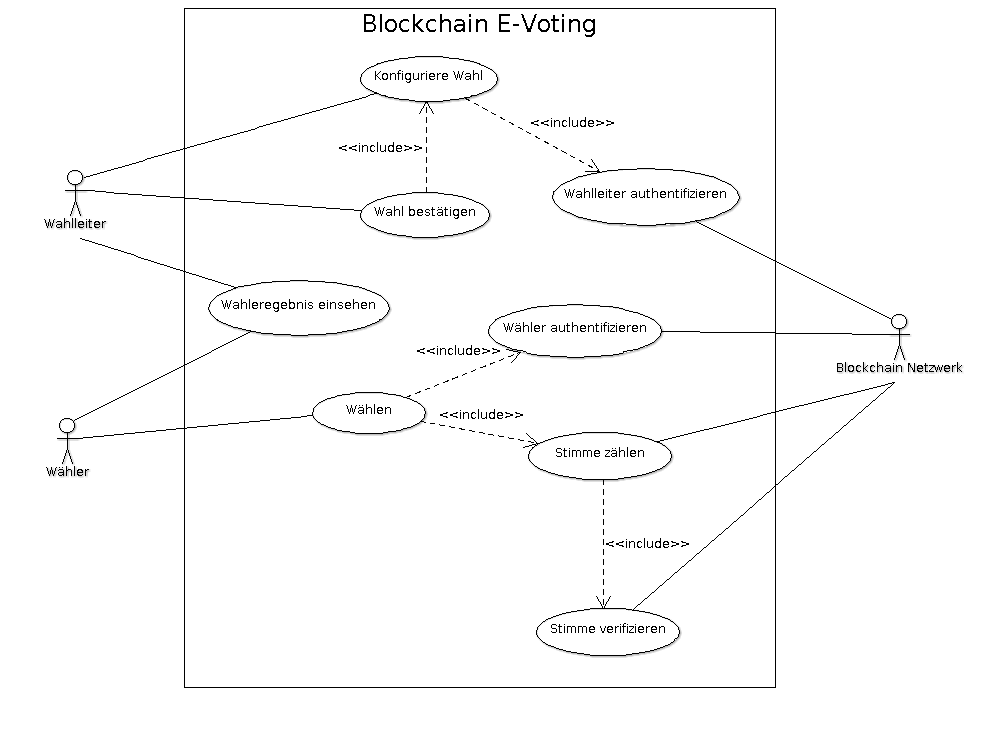
\includegraphics[width=\textwidth]{res/UseCaseDiagram.png}}
	\caption{\label{fig:usecase}
		Ein Use-Case-Diagramm mit den typischen Funktionen der Software.
	}
\end{figure}

\subsection{Netzwerk}
\begin{figure}[H]
	\fbox{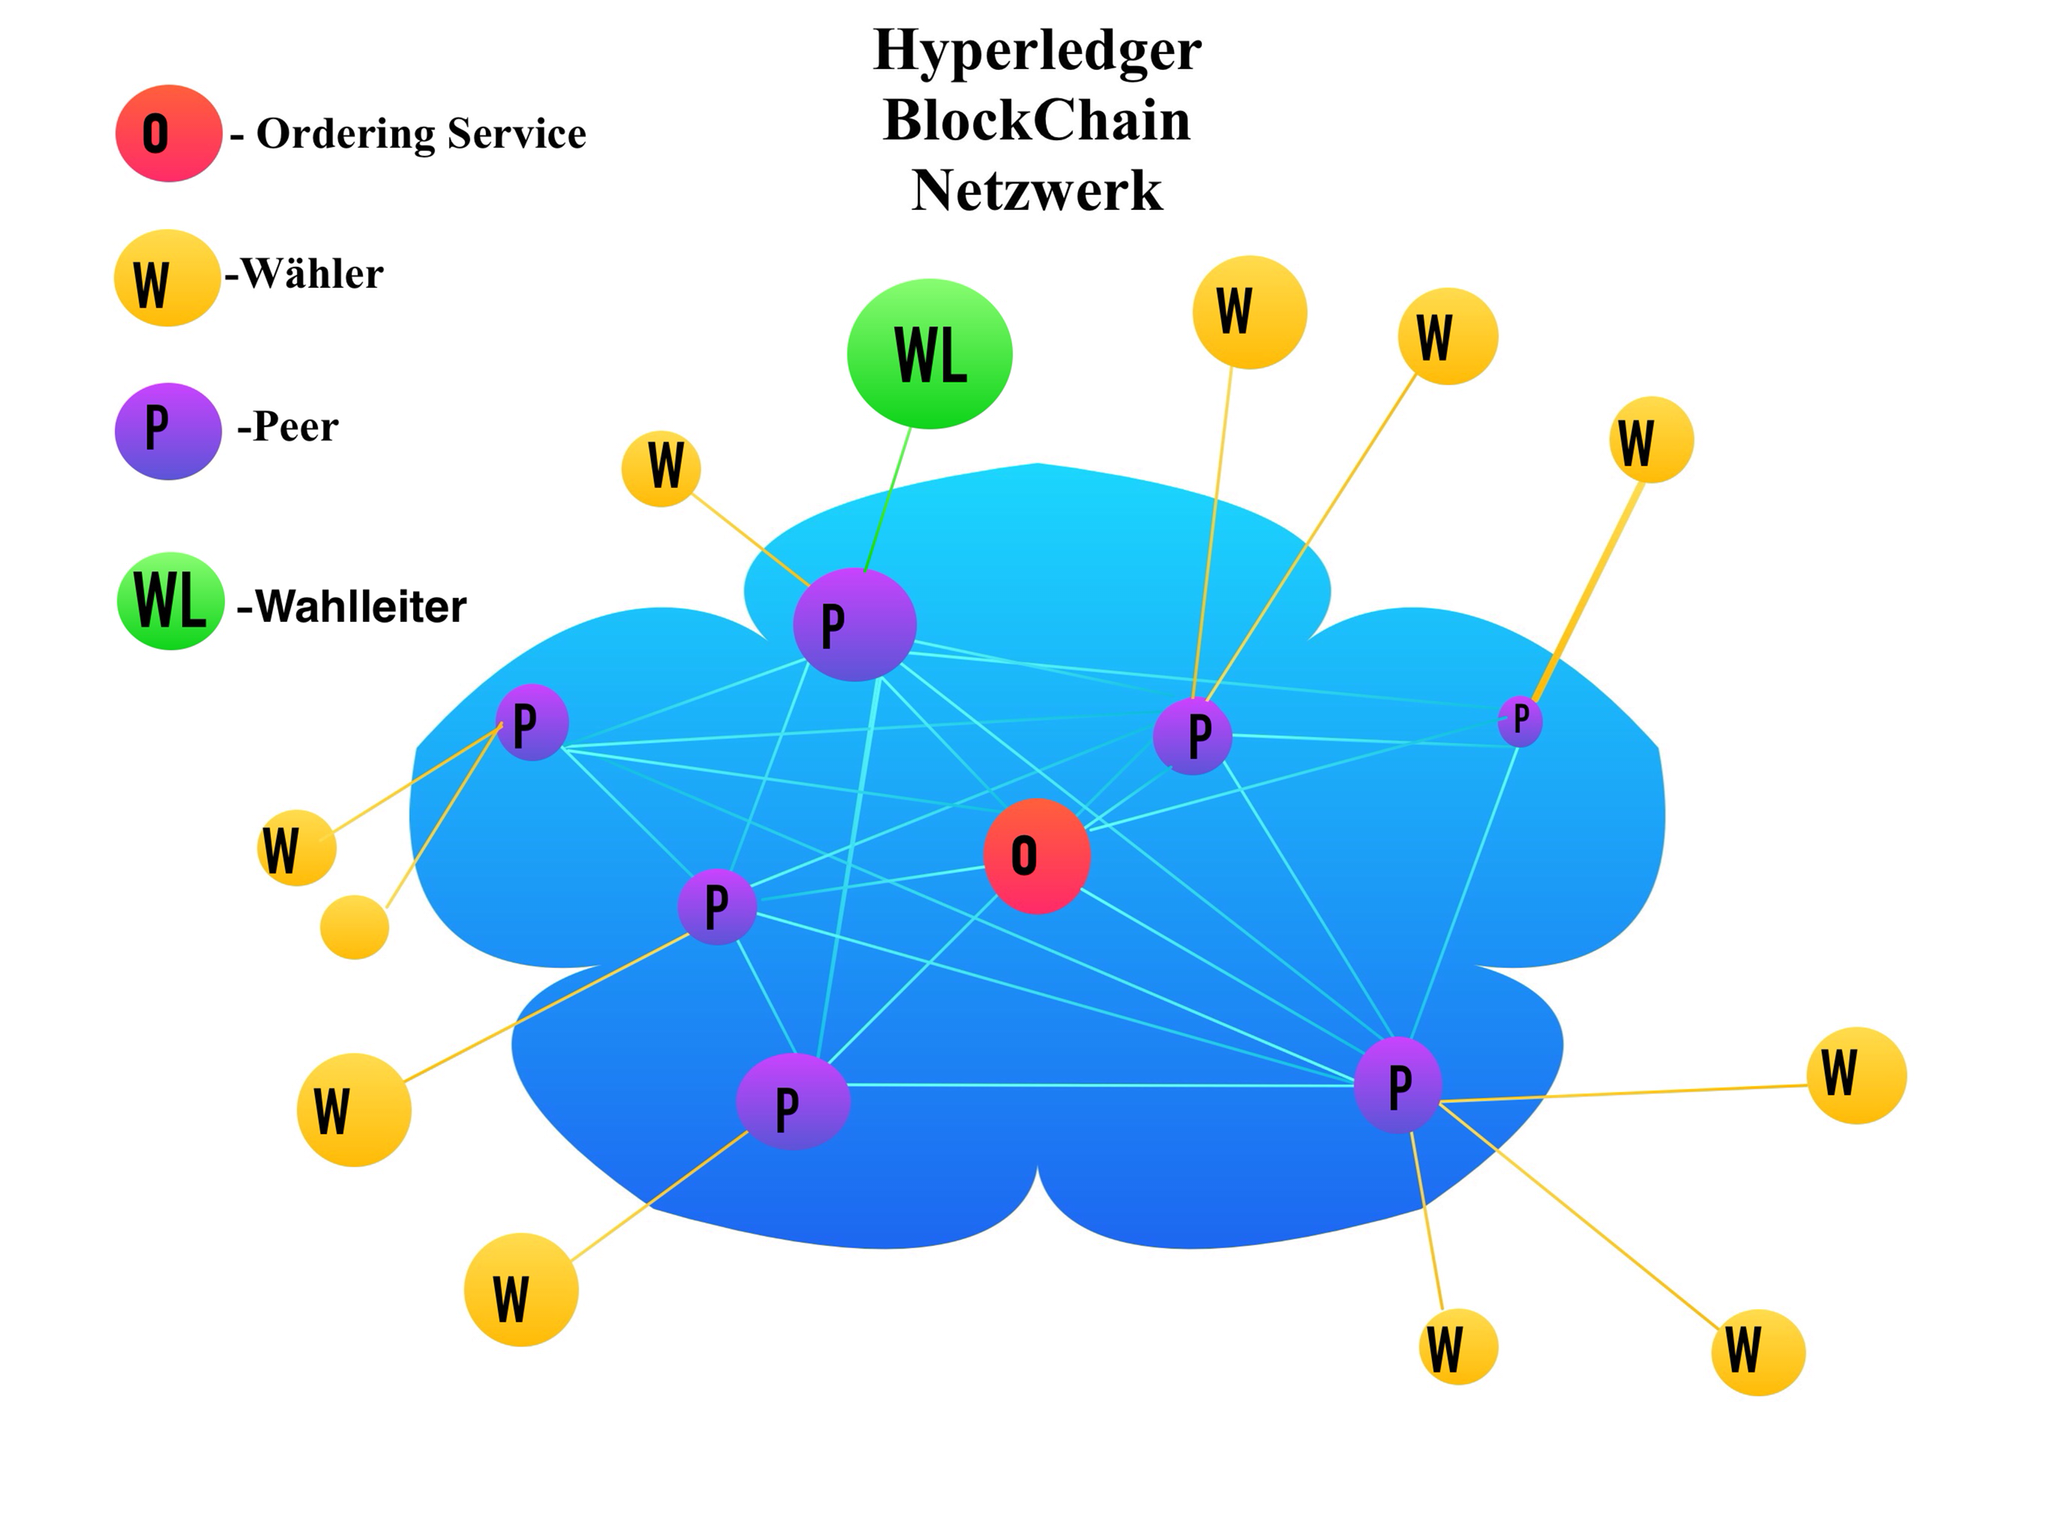
\includegraphics[width=\textwidth]{res/netzwerk_topologie.jpg}}
	\caption{\label{fig:network}
		Darstellung des Blockchain Netzwerkes.
	}
\end{figure}

\section{Benutzeroberfläche}

\subsection{Wahlleiter}

\begin{figure}[H]
	\fbox{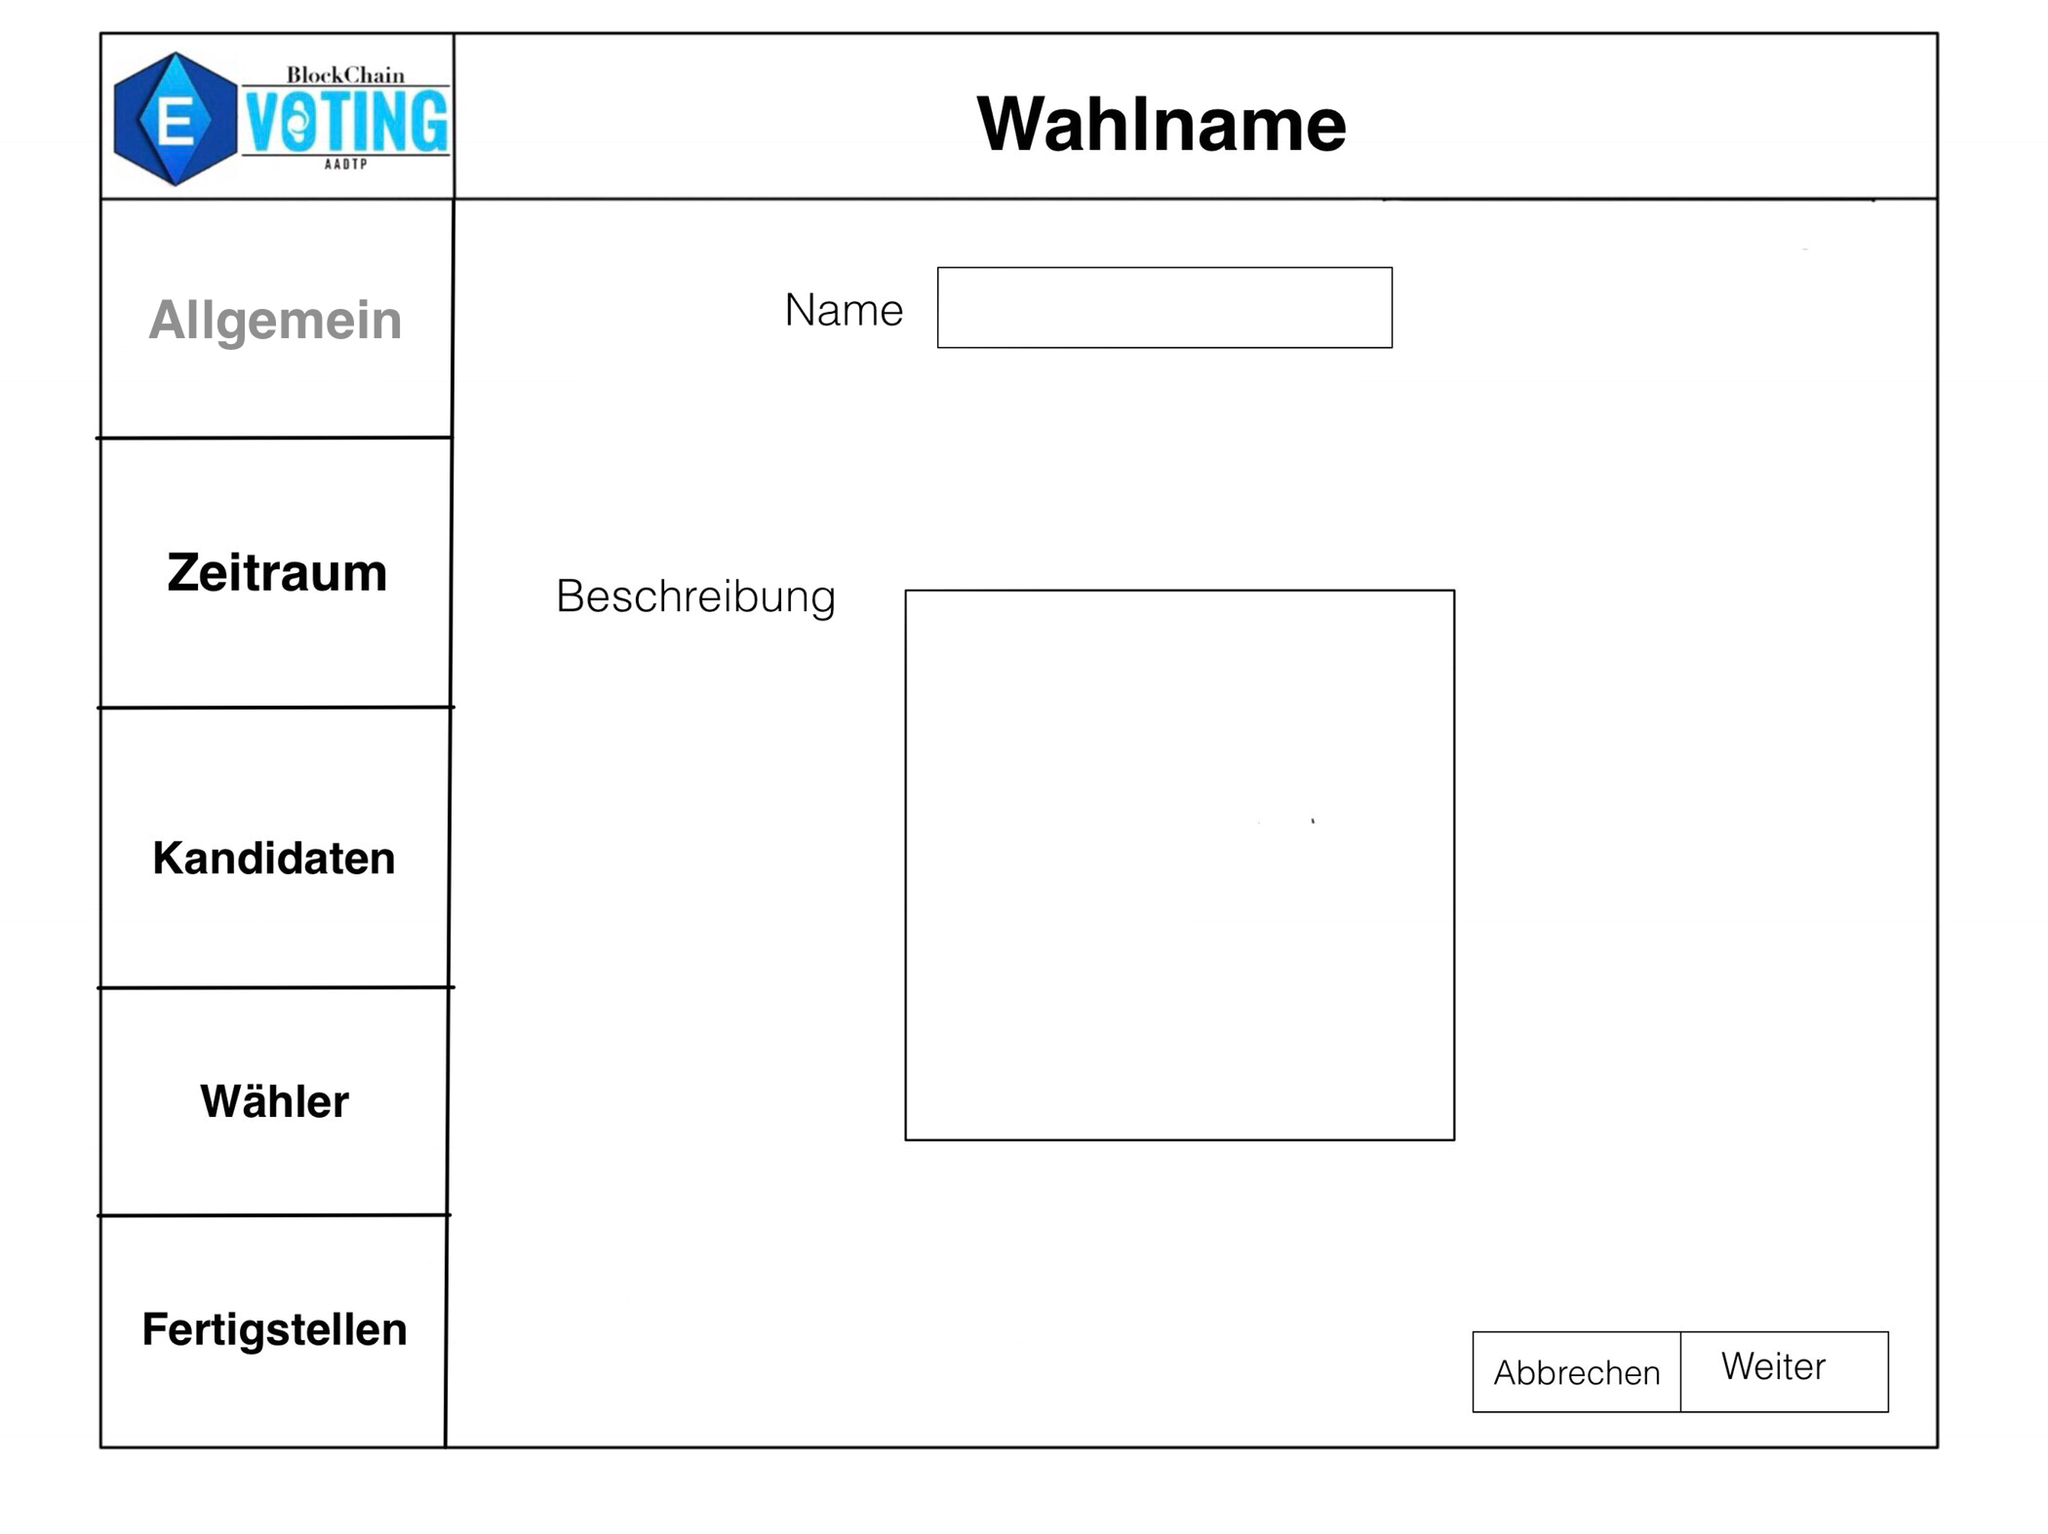
\includegraphics[width=\textwidth]{res/wahlleiter_allgemein.jpg}}
	\caption{\label{fig:wlltr-general}
		Allgemeine Einstellungen einer Wahl.
	}
\end{figure}
Der Wahlleiter kann einen Namen für die Wahl vergeben und das zu verwendende Wahlsystem auswählen.
Er kann der Wahl eine Beschreibung hinzufügen.
Bei betätigen des weiter Buttons wechselt er zum nächsten Schritt der Wahlkonfiguration.
%Die Angabe eines Namens und Wahlsystems sind hierbei notwendig um fortzufahren.

\begin{figure}[H]
	\fbox{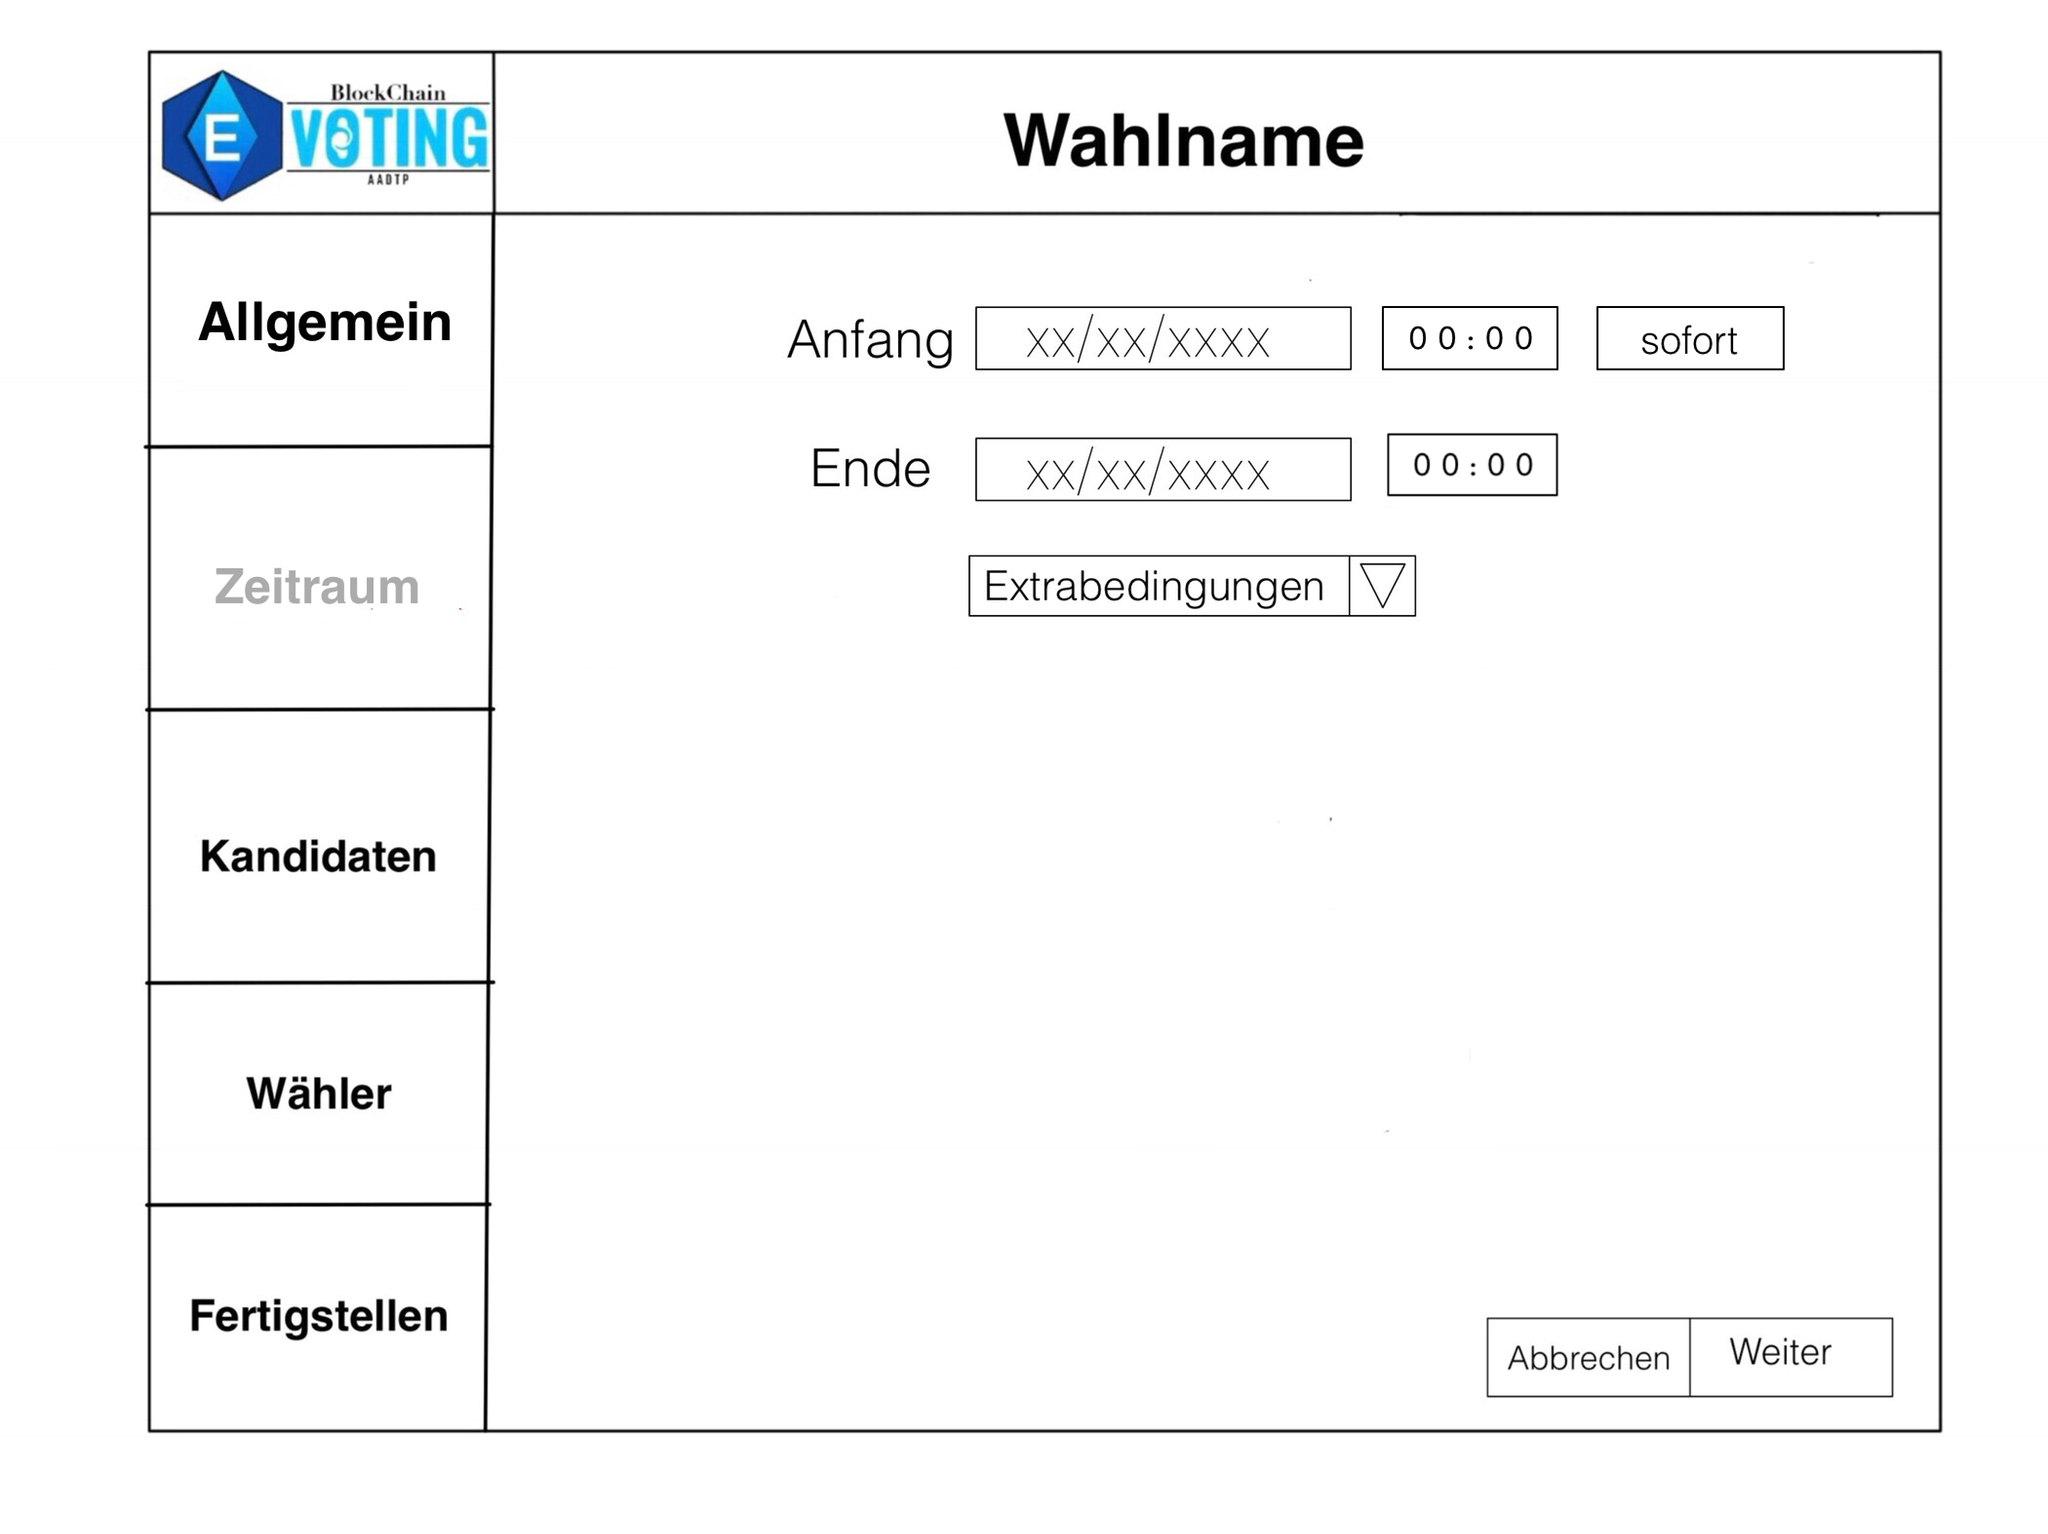
\includegraphics[width=\textwidth]{res/wahlleiter_zeitraum.jpg}}
	\caption{\label{fig:wlltr-time}
		Einstellungen um den Zeitraum der Wahl zu bestimmen.
	}
\end{figure}
Der Wahlleiter kann den Anfang und das Ende des Wahlvorgangs bestimmen.
%Sowohl das Anfangs als auch das Ende des Wahlvorgangs müssen angegeben sein um fortzufahren.

\begin{figure}[H]
	\fbox{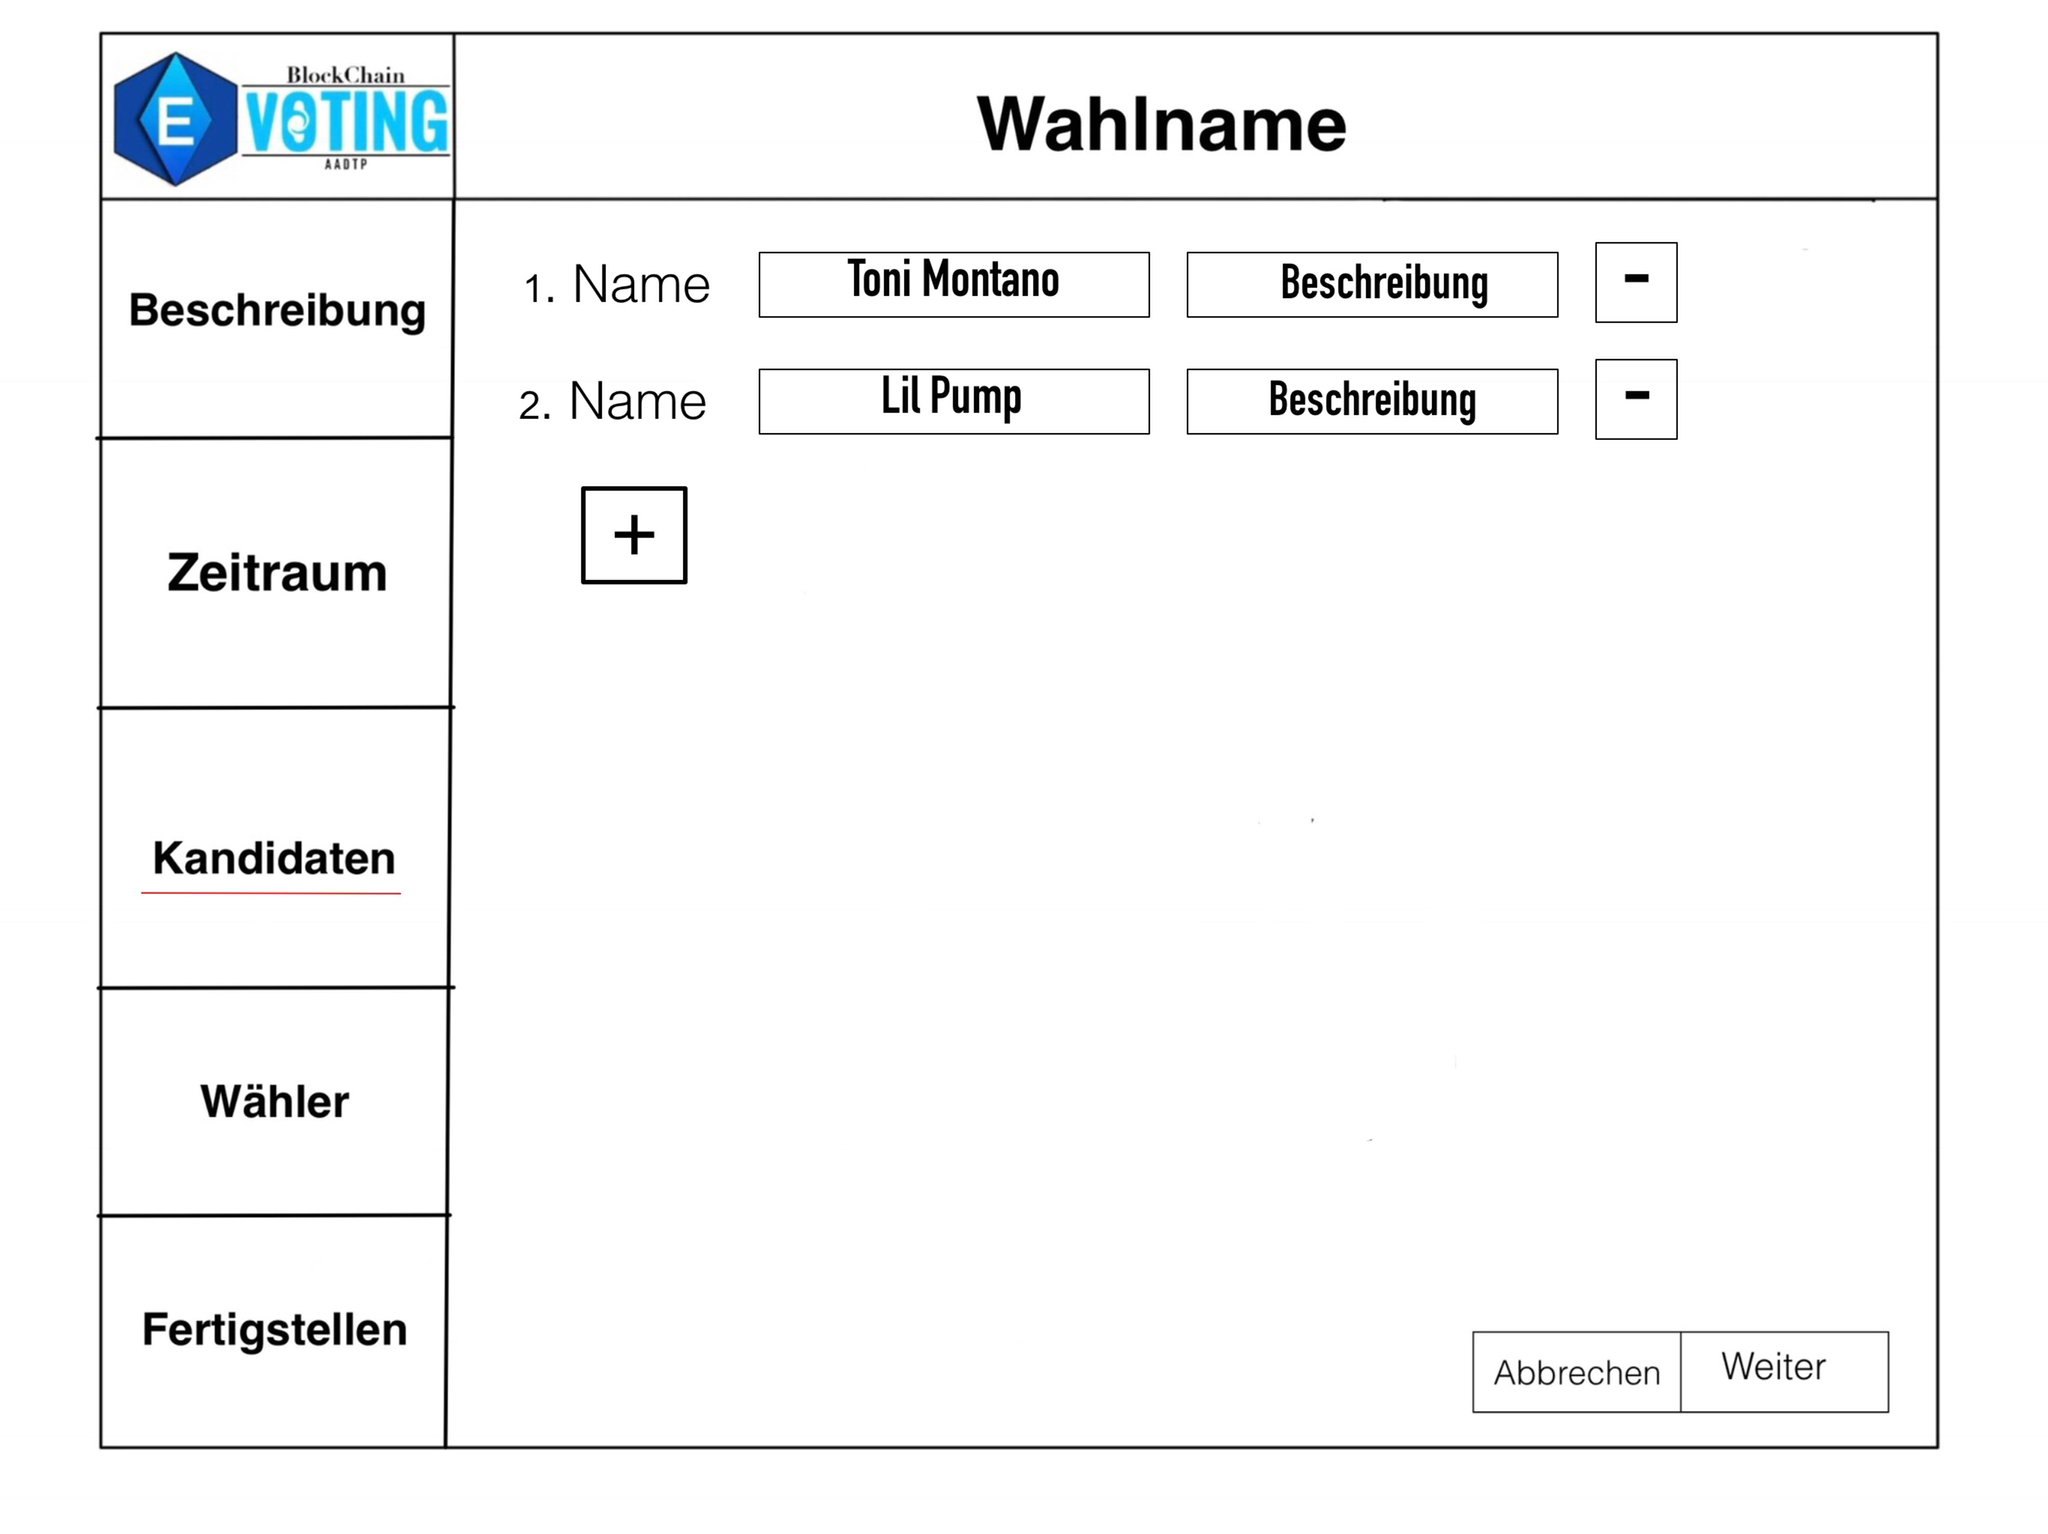
\includegraphics[width=\textwidth]{res/wahlleiter_kandidaten.jpg}}
	\caption{\label{fig:wlltr-candidate}
		Hinzufügen der \glslink{Kandidat}{Kandidaten}.
	}
\end{figure}
Der Wahlleiter kann durch betätigen des ''+'' Buttons Kandidaten zur Wahl hinzufügen.
Er kann Kandidaten einen Namen und eine Beschreibung vergeben.
Durch das betätigen des ''-'' Buttons an einem Kandidaten wird dieser von der Wahl entfernt.
%Jeder Kandidat benötigt einen angegeben Namen um fortzufahren. Angebung einer Beschreibung ist optional.

\begin{figure}[H]
	\fbox{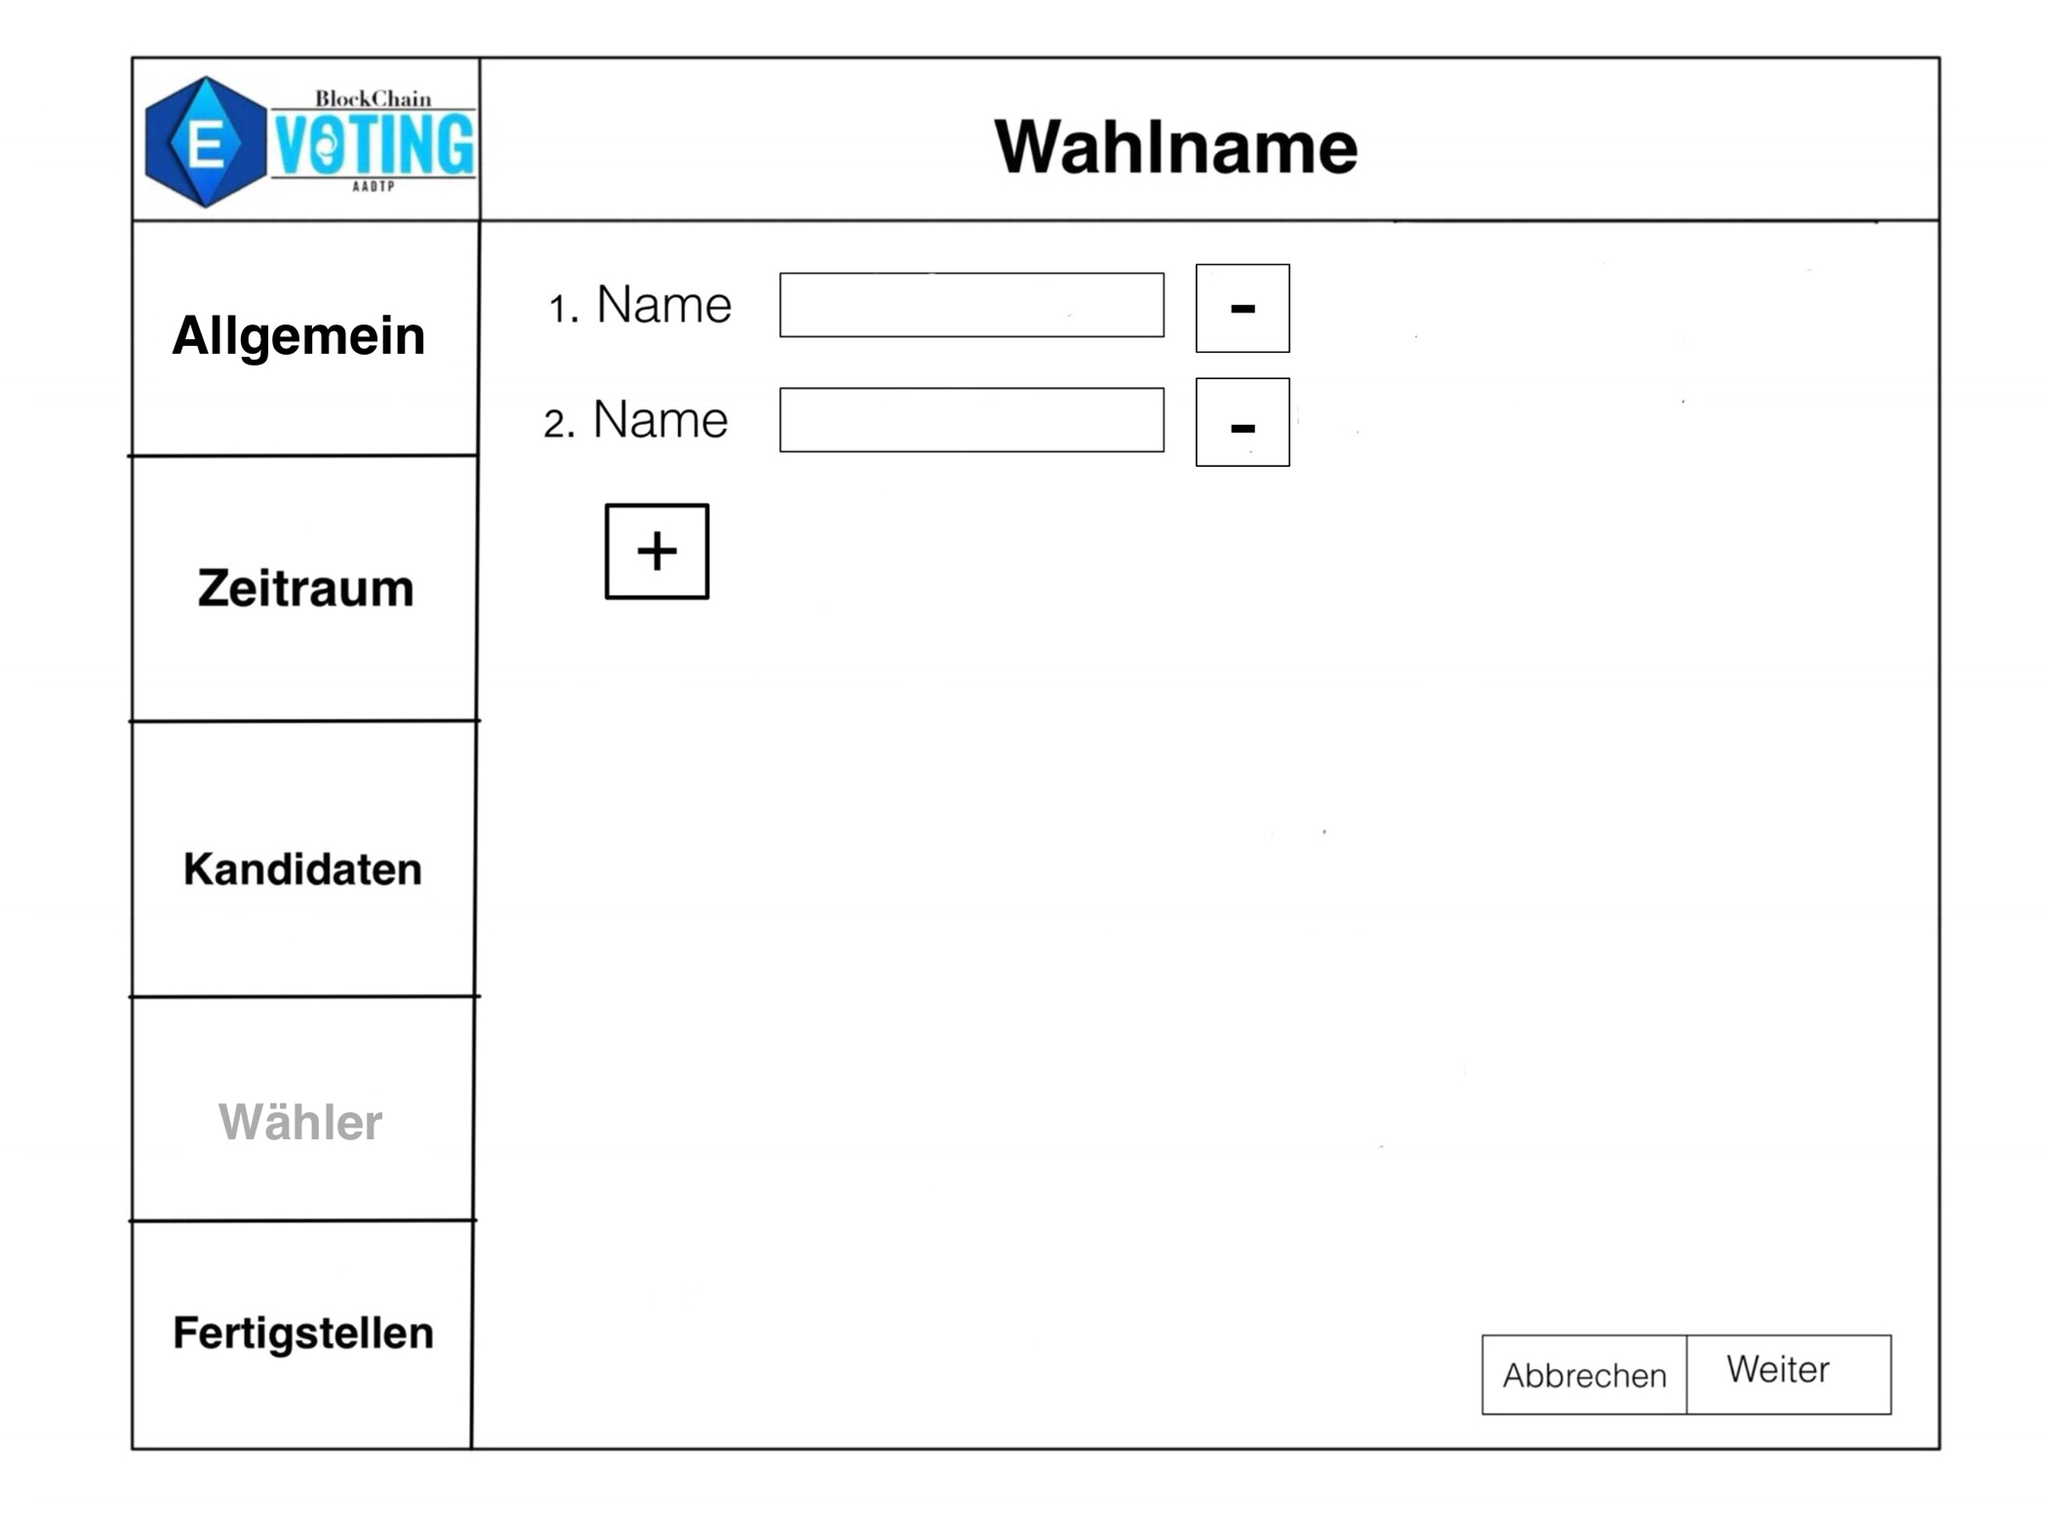
\includegraphics[width=\textwidth]{res/wahlleiter_waehler.jpg}}
	\caption{\label{fig:wlltr-voter}
		Hinzufügen der \gls{Waehler}.
	}
\end{figure}
Der Wahlleiter kann nach gleichem Prinzip Wähler hinzufügen und entfernen.
Er kann hierbei die Namen der Wähler angeben.
%Alternativ: Der Name eines jeden Wählers muss angegeben sein um fortzufahren.

\begin{figure}[H]
	\fbox{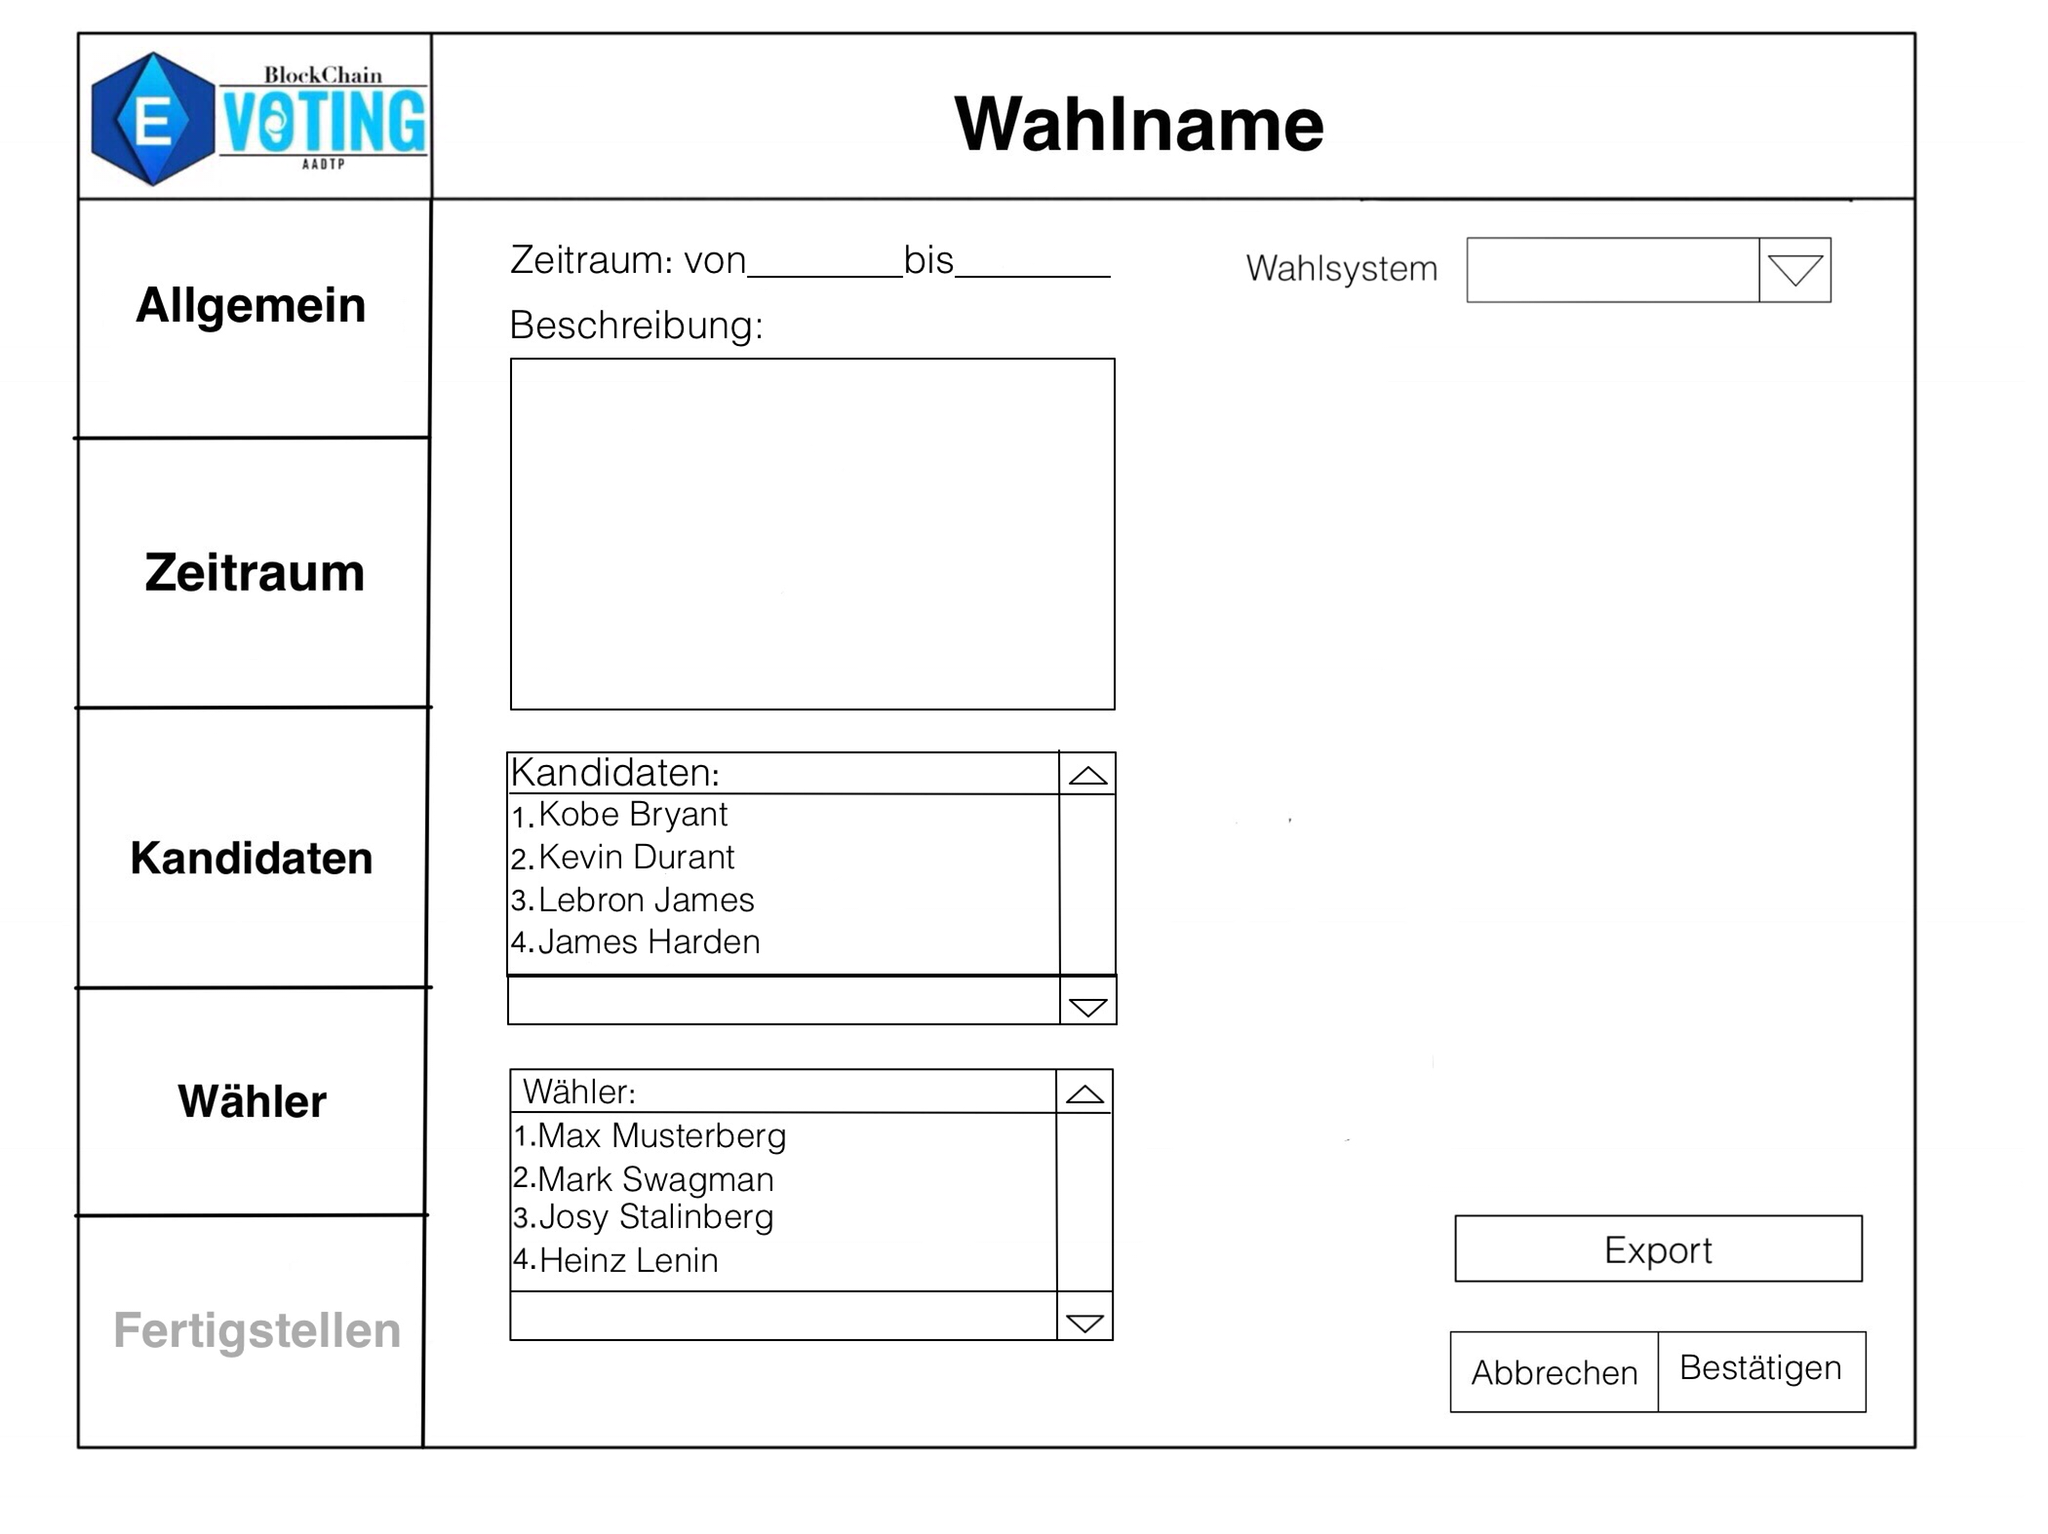
\includegraphics[width=\textwidth]{res/wahlleiter_fertig.jpg}}
	\caption{\label{fig:wlltr-done}
		Übersicht über alle Einstellungen.
	}
\end{figure}
Der Wahlleiter sieht alle vorgenommenen Einstellungen seiner Wahl:
\begin{enumerate}
	\item Den Start- und Endzeitpunkt der Wahl
	\item Alle zur Wahl verfügbar stehenden Kandidaten inkl. Name und Beschreibung.
	\item Alle zur Wahl berechtigten Wähler und deren Namen.
\end{enumerate}
Bei betätigen des ''export'' Buttons kann der Wahlleiter die Konfiguration der Wahl speichern.
Bei betätigen des ''weiter'' Buttons wird die Wahl erstellt.

\begin{figure}[H]
	\fbox{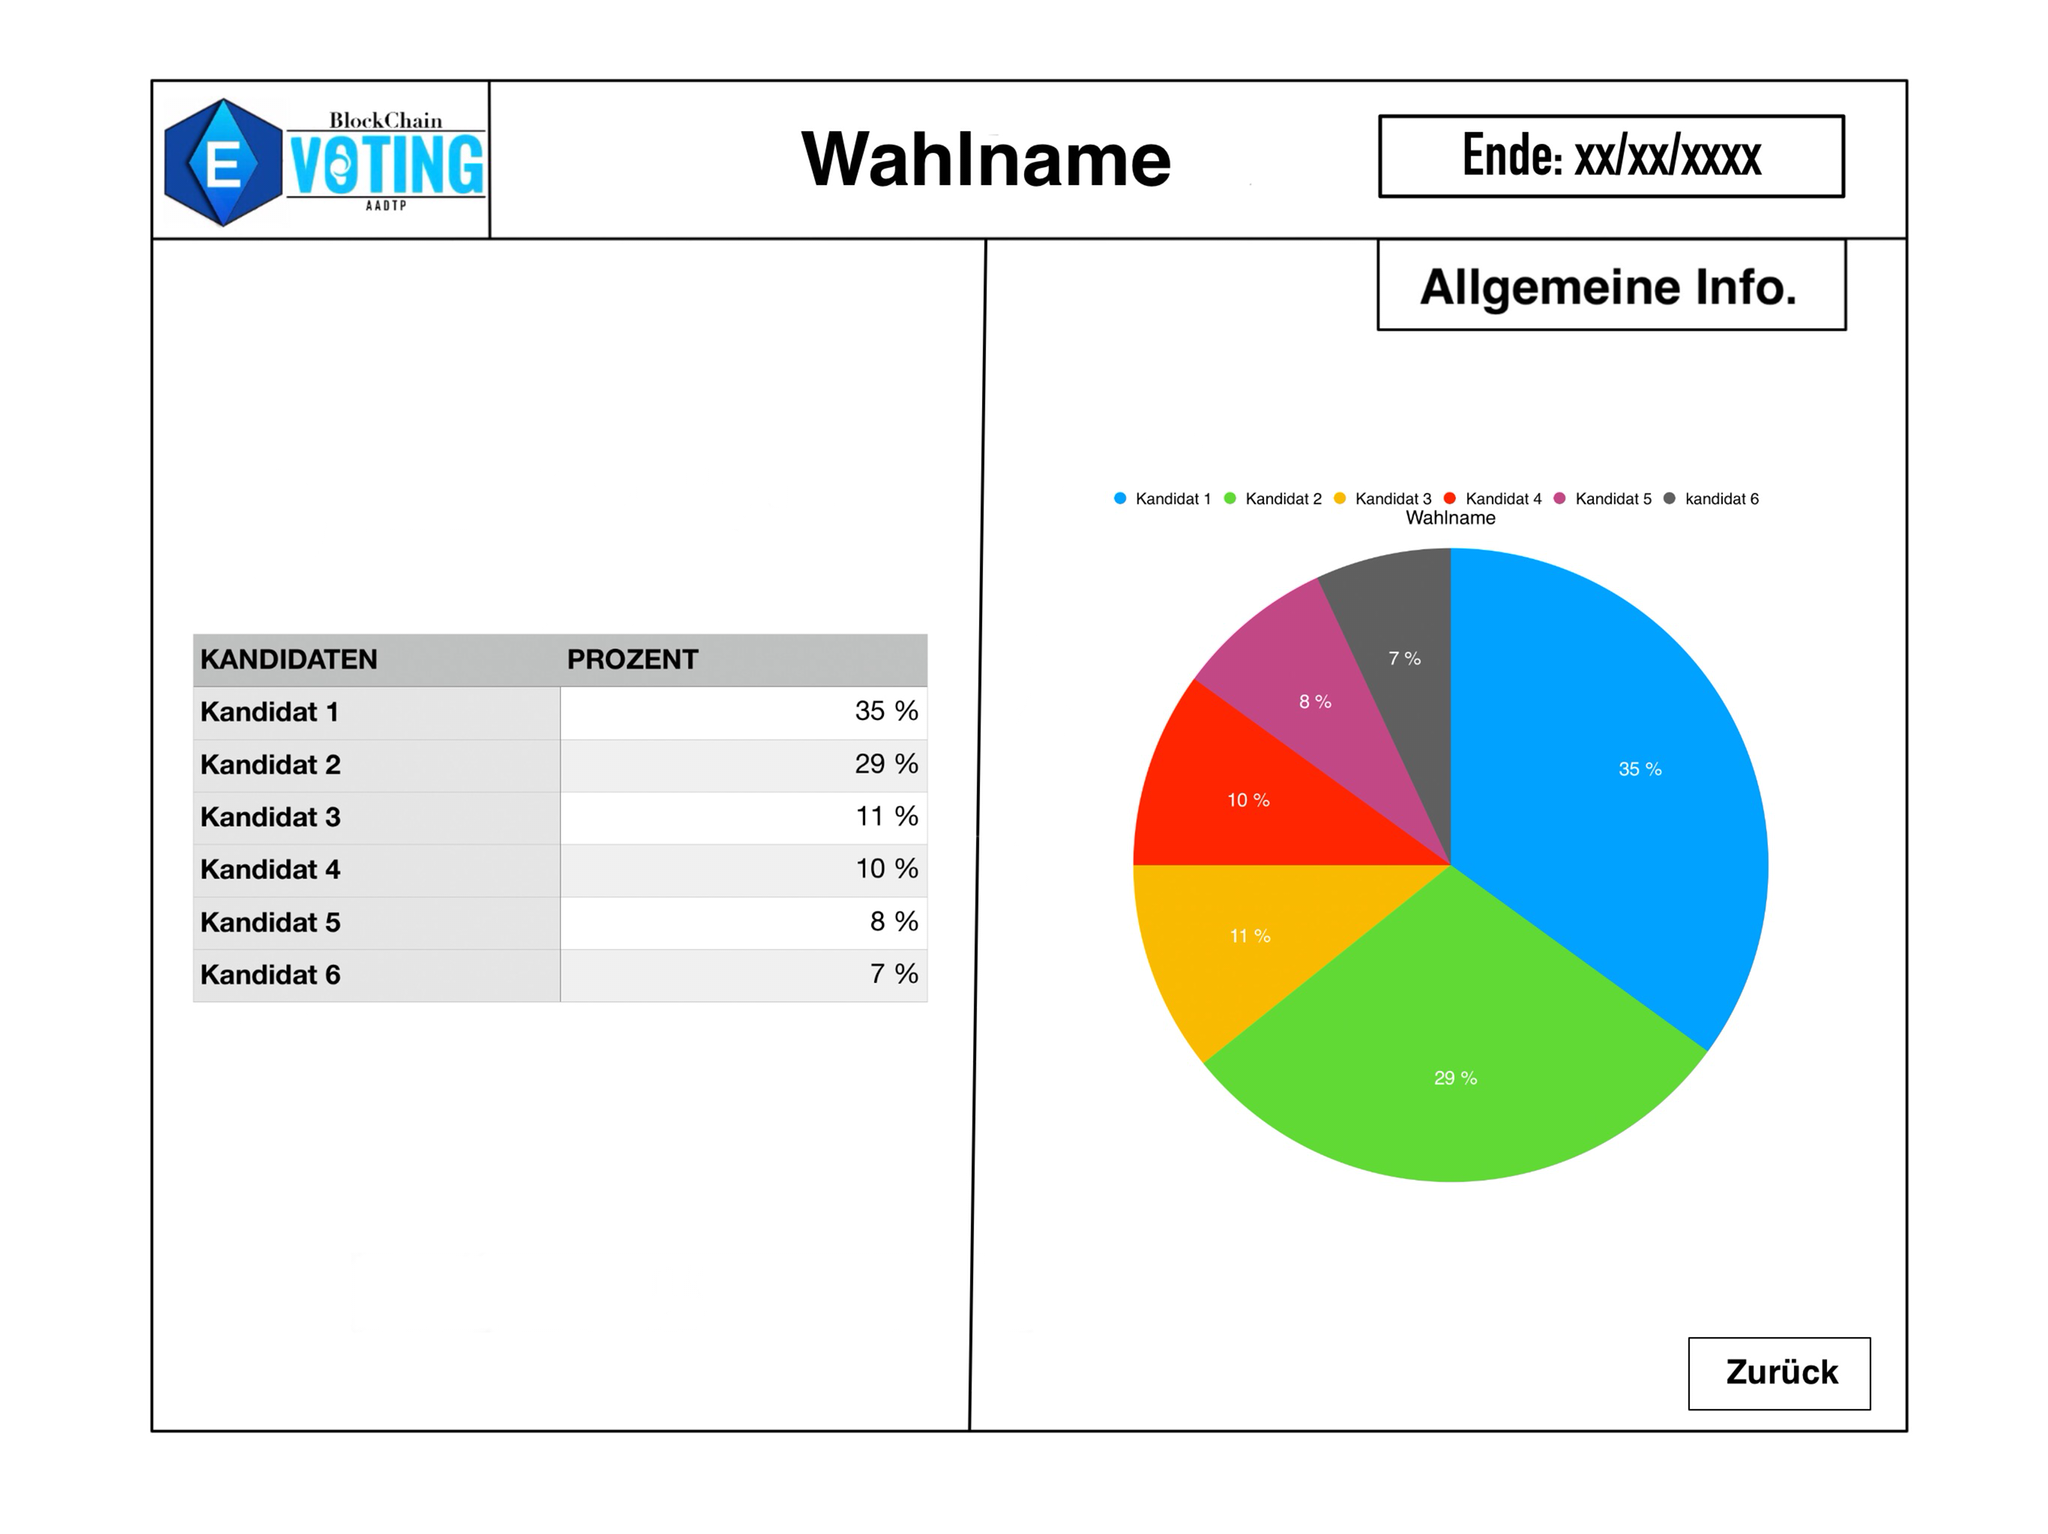
\includegraphics[width=\textwidth]{res/wahlleiter_status.jpg}}
	\caption{\label{fig:wlltr-status}
		Übersicht über den aktuellen Wahlstand.
	}
\end{figure}
Der Wahlleiter bekommt während dem Ablauf der Wahl tabellarisch und in Form eines Diagrammes den aktuellen Stand seiner Wahl dargestellt.


\subsection{Wähler}

\begin{figure}[H]
	\fbox{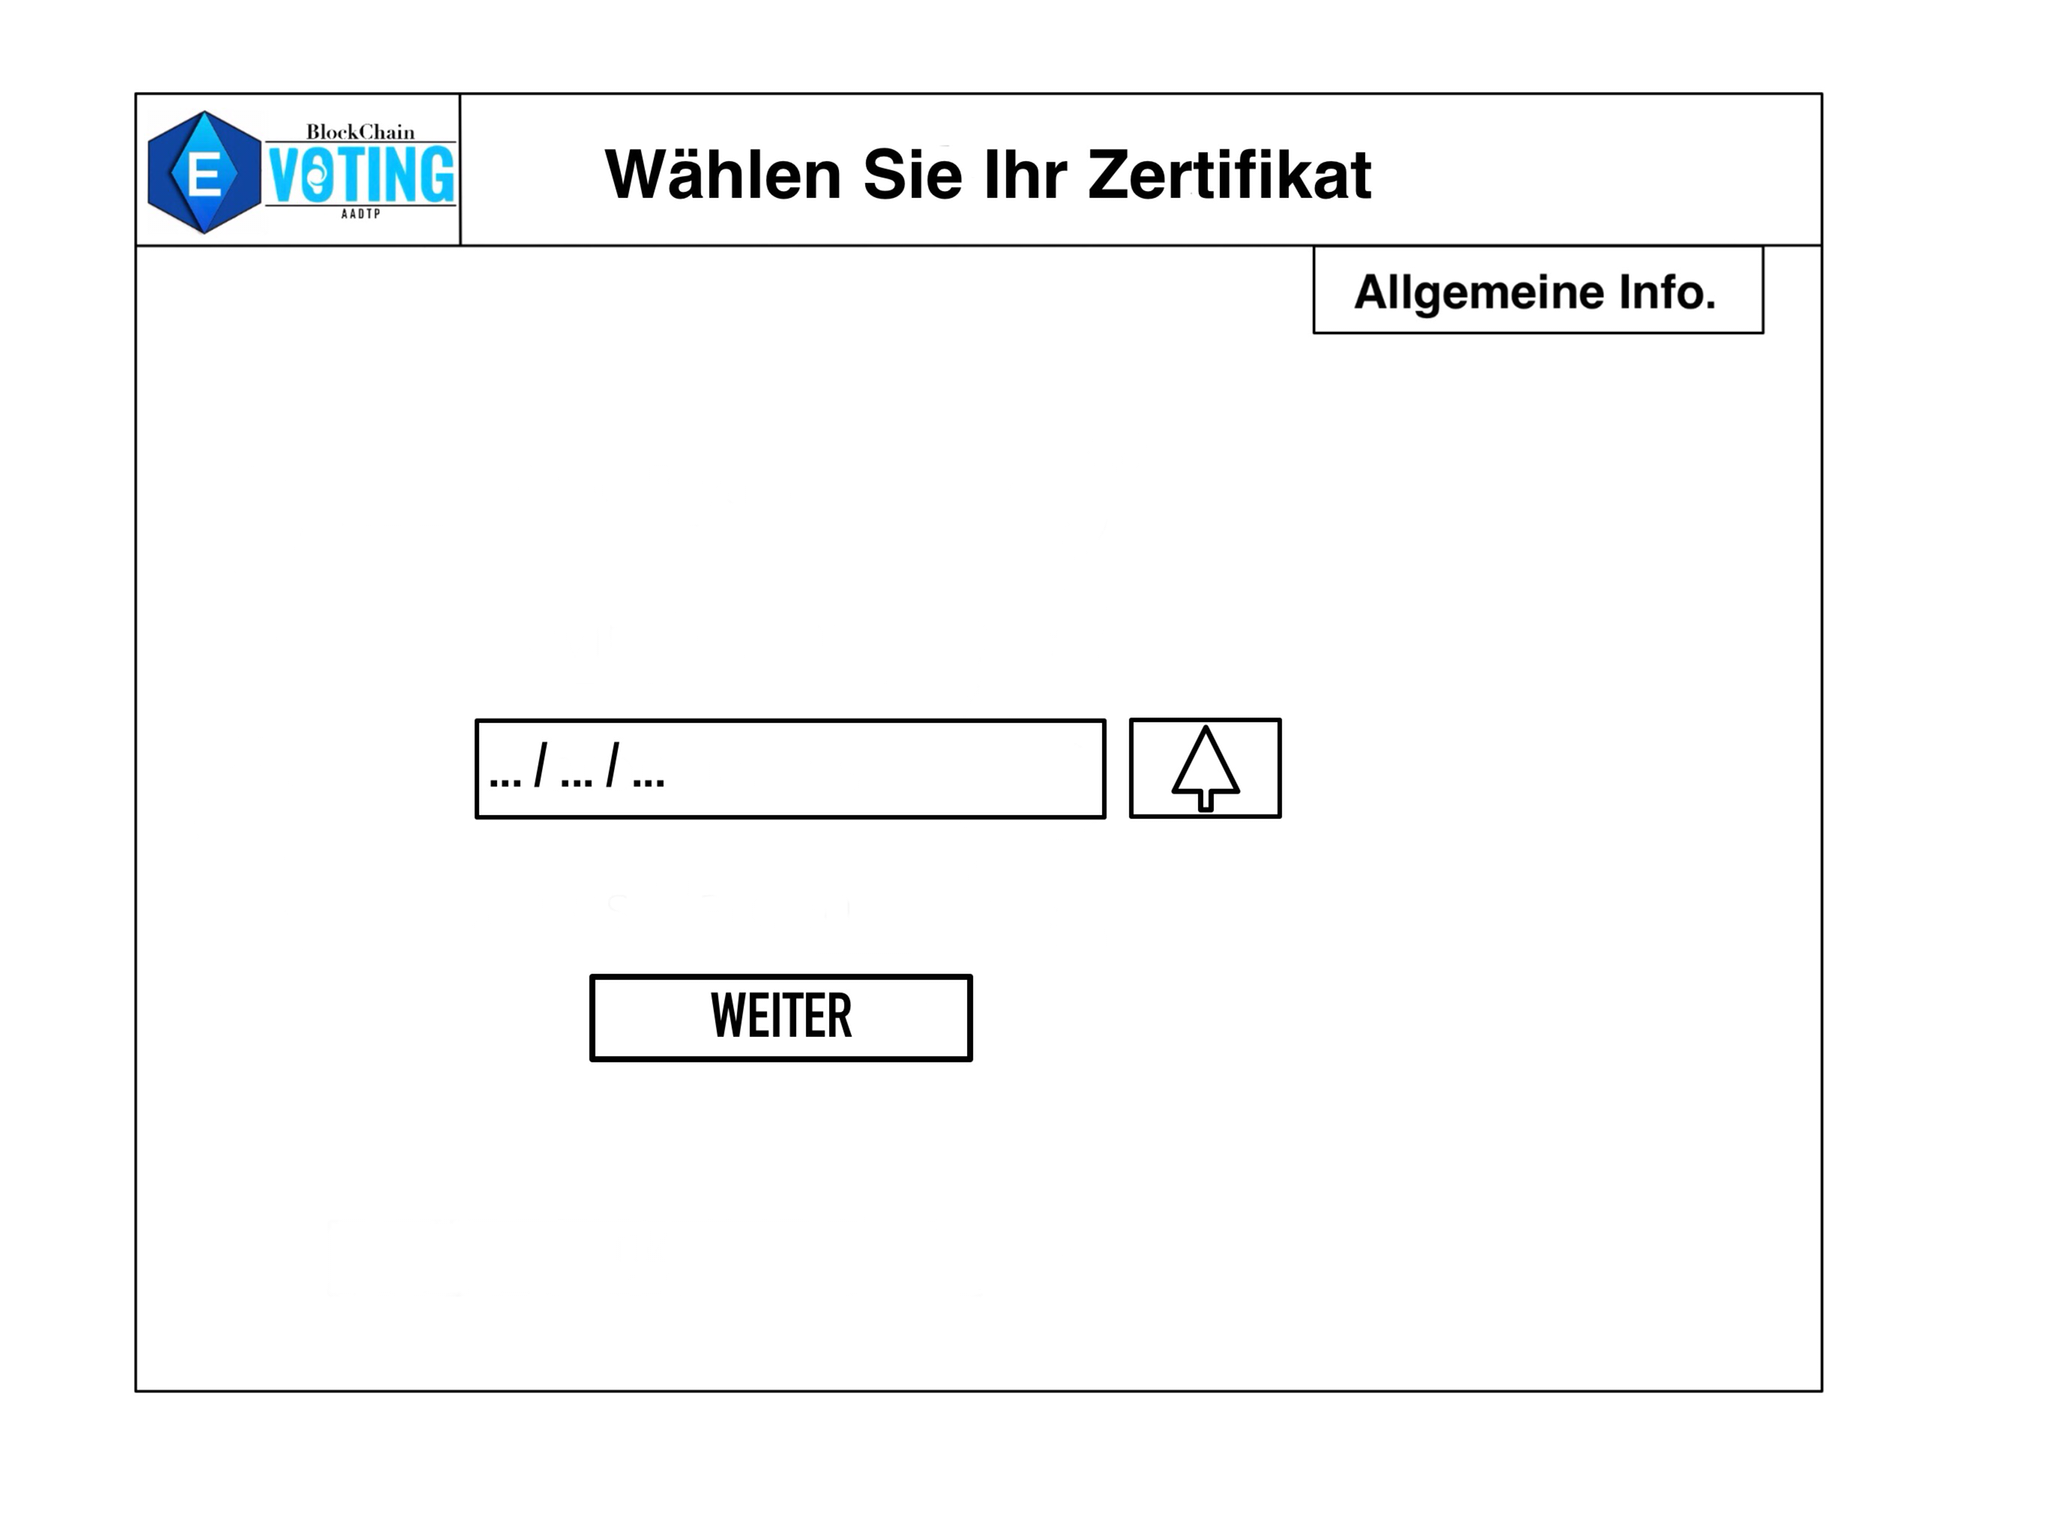
\includegraphics[width=\textwidth]{res/waehler_start.jpg}}
	\caption{\label{fig:whlr-start}
		Anfangs-GUI die das Zertifikat des Wählers anfragt.
	}
\end{figure}
Der Wähler kann in seinem Dateibrowser das Zertifikat auswählen und mit betätigen des weiter Buttons zur Wahl fortschreiten.

\begin{figure}[H]
	\fbox{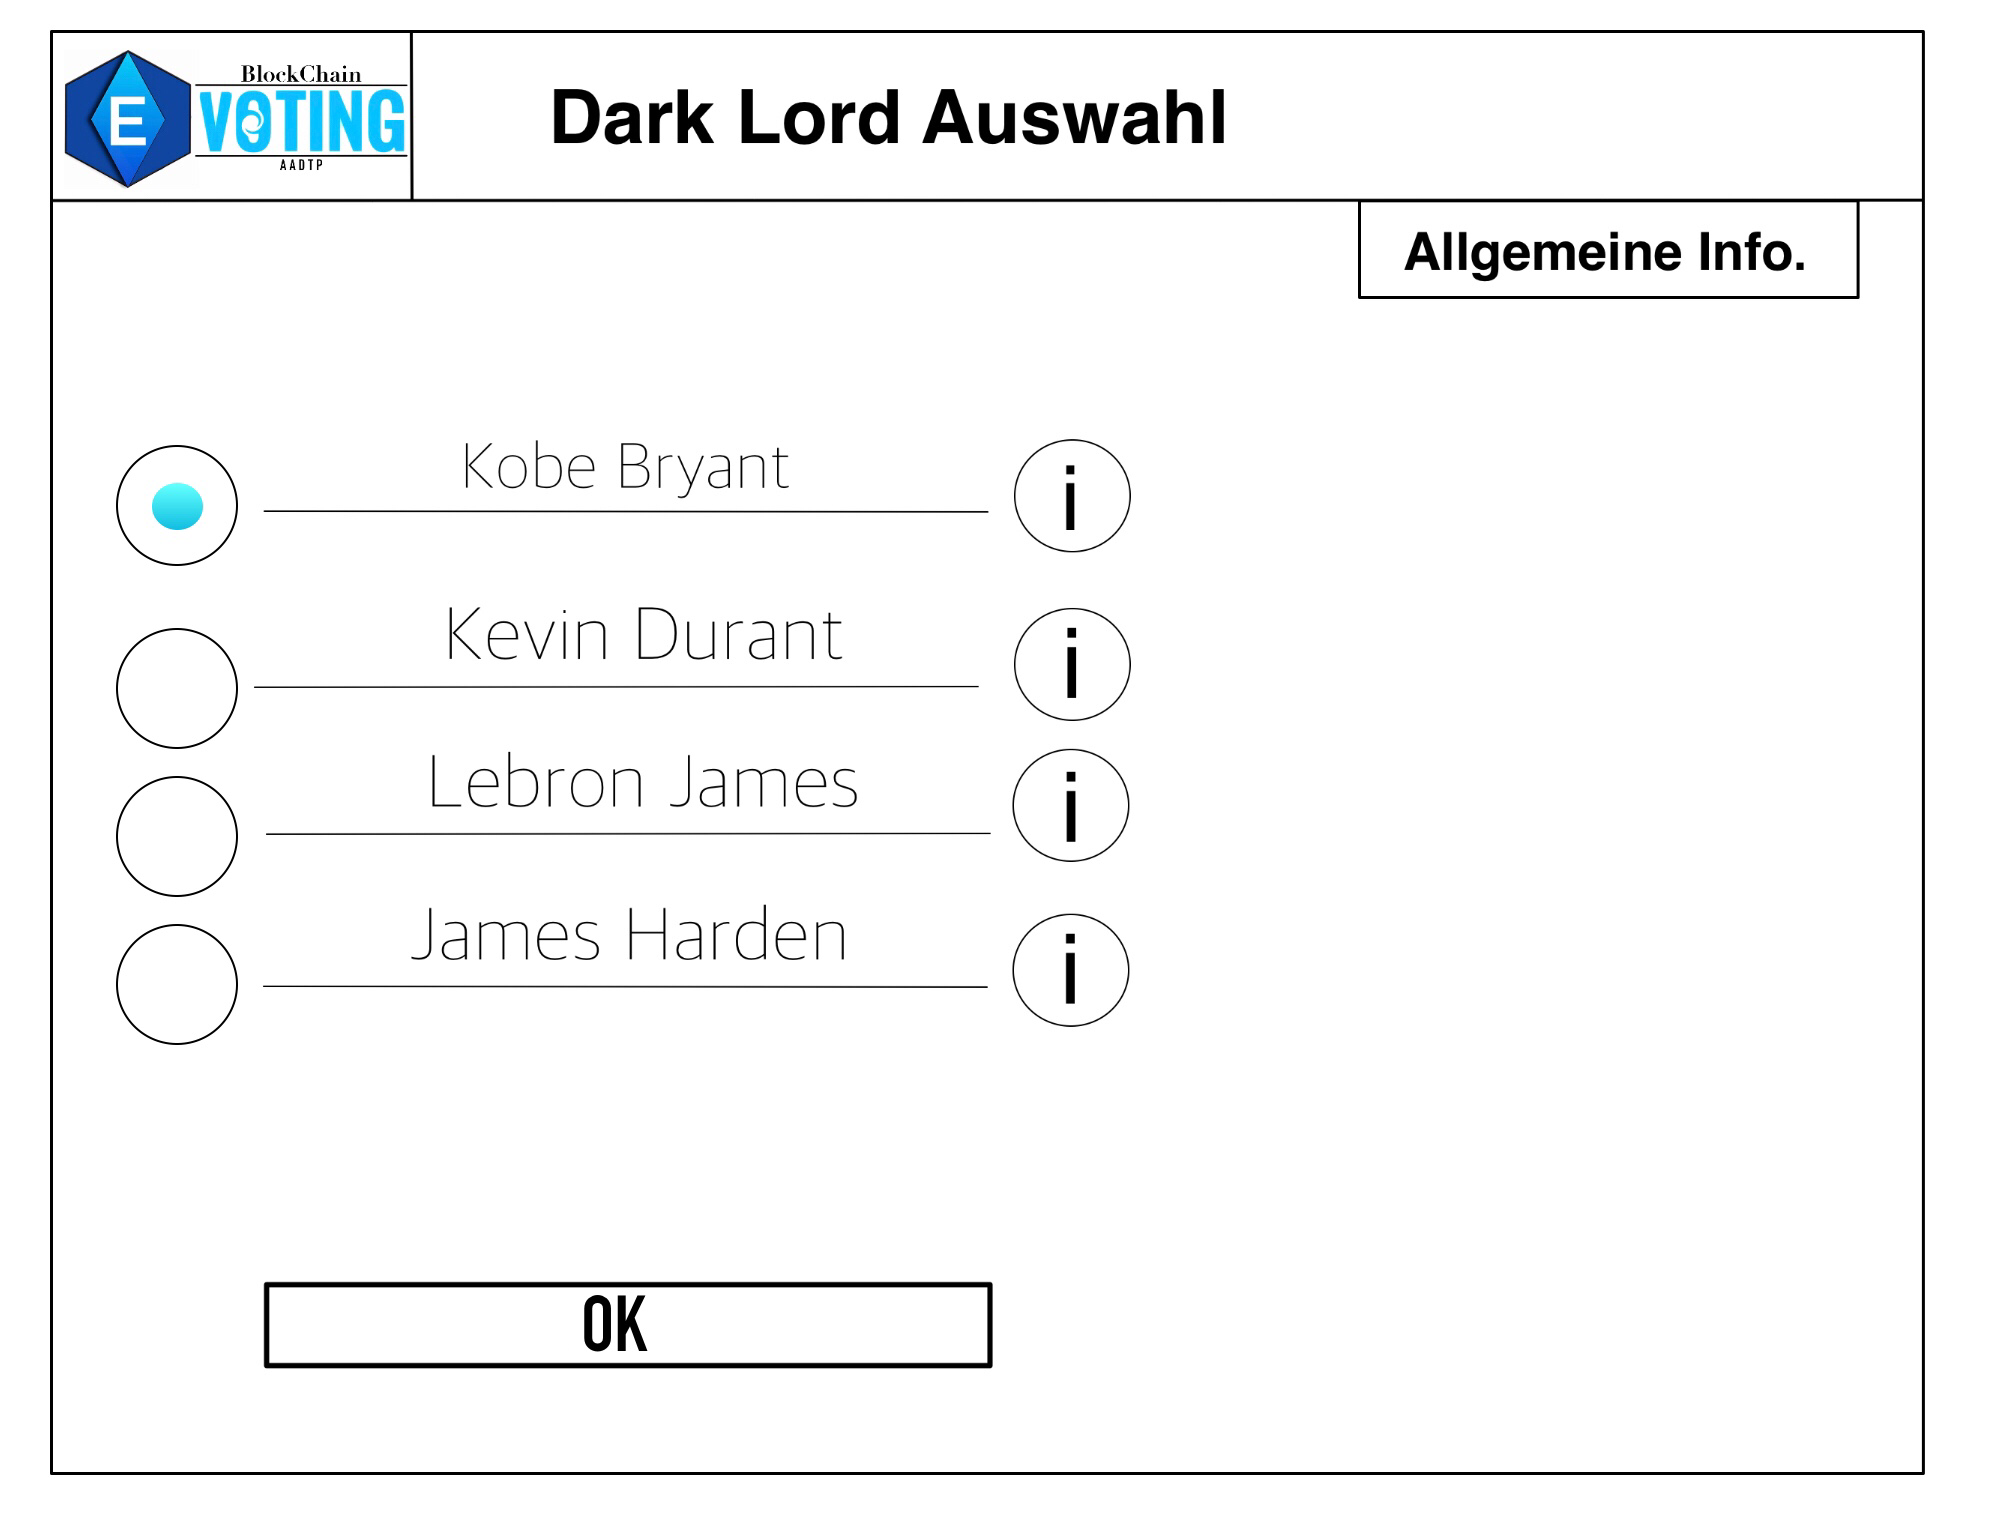
\includegraphics[width=\textwidth]{res/waehler_wahl.jpg}}
	\caption{\label{fig:whlr-wahl}
		Auswahl der Kandidaten.
	}
\end{figure}
Der Wähler kann einen oder mehrere Kandidaten auswählen und seine Auswahl beliebig oft ändern.
Das anwählen des ''i'' Buttons zeigt die Beschreibung des entsprechenden Kandidaten.
Bei betätigen des ''OK'' Buttons wird die Wahl bestätigt.


\begin{figure}[H]
	\fbox{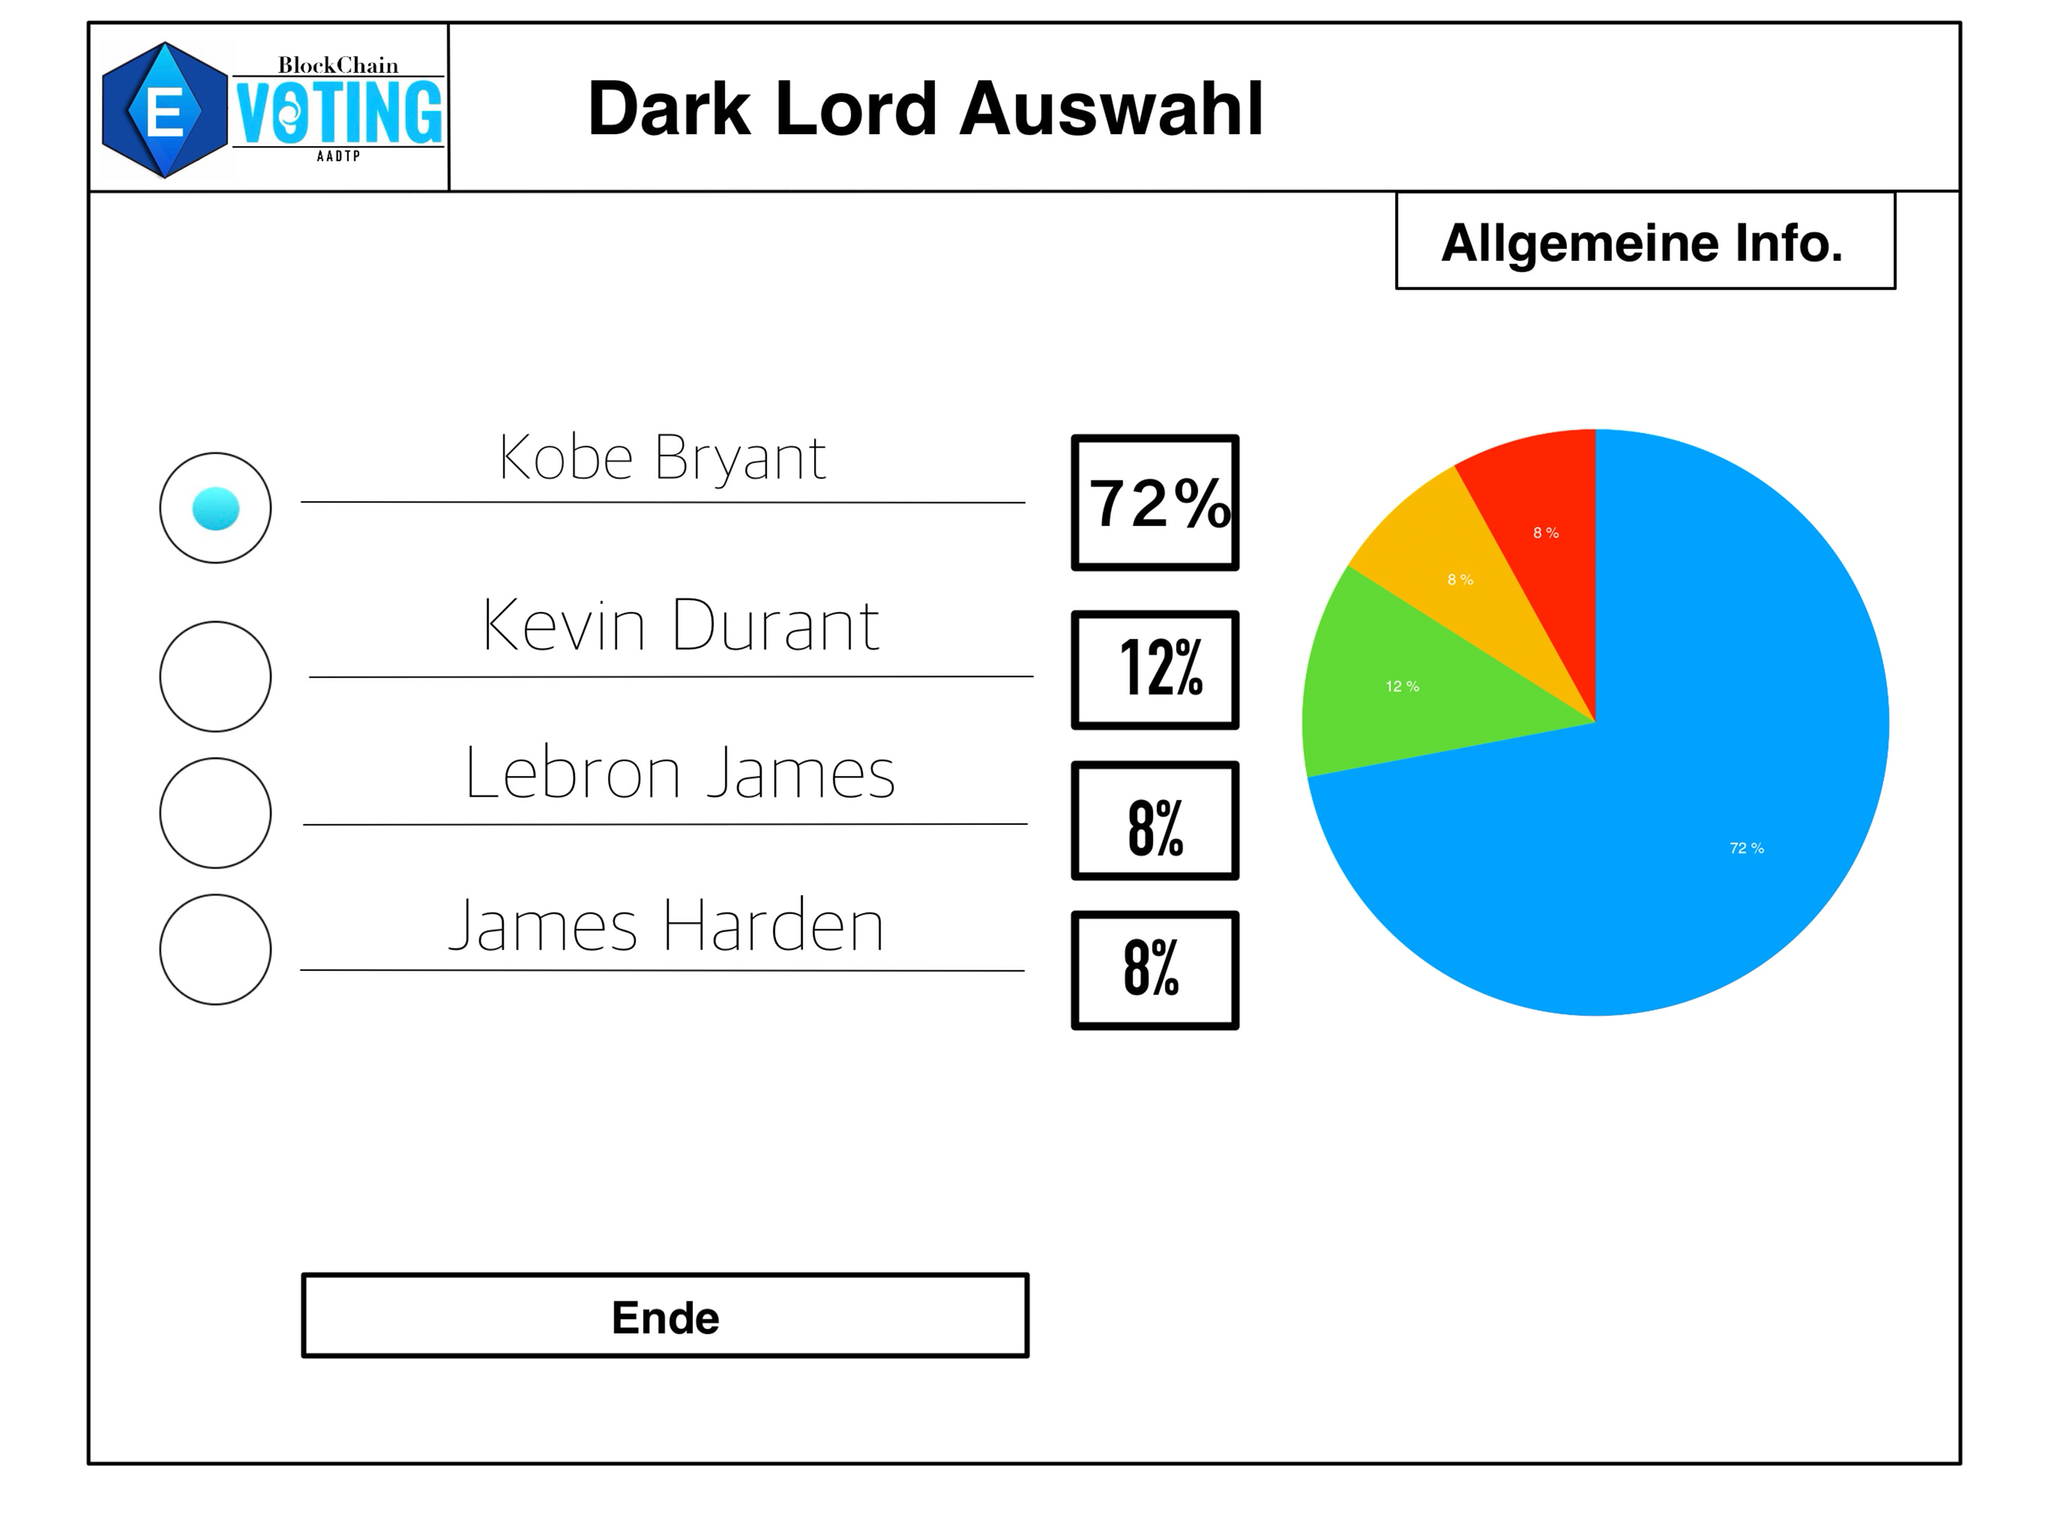
\includegraphics[width=\textwidth]{res/waehler_result.jpg}}
	\caption{\label{fig:whlr-result}
		Ergebnisse der Wahl.
	}
\end{figure}
Der Wähler kann seine abgegebene Auswahl einsehen.
Sobald der Wahlvorgang beendet wird sieht er zusätzlich die Ergebnisse der Wahl.

\section{Spezielle Anforderungen an die Entwicklungsumgebung}
Zur Entwicklung werden die IntelliJ oder Eclipse IDE verwendet.
Zudem wird ein \gls{Linux} basiertes Betriebssystem verwendet.

\section{Glossar}
\printglossaries

\end{document}
